\documentclass[10pt]{scrreprt}
\usepackage[a4paper, top=30mm, left=25mm, right=25mm, bottom=30mm]{geometry}
\usepackage[utf8]{inputenc}

\usepackage[Bjornstrup]{fncychap}
\usepackage{ngerman}
\usepackage{graphicx}
\usepackage{epstopdf}
\usepackage{etoolbox}
\usepackage{enumitem}
\usepackage{url}
\usepackage{numprint}
\usepackage{longtable}
\usepackage{tabu}
\usepackage{caption}
 \usepackage{rotating}
\usepackage{array}
\usepackage{listings}
\usepackage{amssymb}


\makeatletter
\patchcmd{\@makechapterhead}{\vspace*{50\p@}}{\vspace*{-20\p@}}{}{}
\patchcmd{\@makeschapterhead}{\vspace*{50\p@}}{\vspace*{7\p@}}{}{}
\patchcmd{\DOTIS}{\vskip 40\p@}{\vskip -12\p@} 
\makeatother
  
\captionsetup[figure]{labelfont={sf,bf},textfont={sf}}
\deffootnotemark{[\thefootnotemark]}
\deffootnote{1.5em}{1em}{[\thefootnotemark] }
\setlength{\parindent}{0pt}
\renewcommand{\labelitemi}{ \raisebox{0.3ex}{\small$\blacktriangleright$} }
\renewcommand{\labelitemii}{ \raisebox{0.3ex}{\small$\triangleright$} }
\lstset{language=Java}

\newcommand{\sfbf}[1]{\textbf{\sffamily #1}}
\newcommand{\sfit}[1]{\textit{\sffamily #1}}
\newcommand{\W}{\sfbf{W}}
\newcommand{\ziel}[1]{{\fontsize{9.5}{11}\textsf{/#1/}}}
\newcommand{\ziellabel}{Z}
\newcommand{\muss}{\renewcommand{\labelenumi}{\textbf{\ziel{\ziellabel\numprint{\theenumi}0}}}}
\newcommand{\wunsch}{\renewcommand{\labelenumi}{\textbf{\ziel{\ziellabel\numprint{\theenumi}0W}}}}
\newcommand{\JoglEarth}{\raisebox{-1.2mm}{
\includegraphics[scale=0.33]{Logo-Text.eps}} }
\newcommand{\textref}[1]{\mbox{\raisebox{0.1ex}{\small$\rightarrow$ }\textit{#1}}}

\newenvironment{details}[1][6pt]{%
  \parskip#1 \parindent6mm \raggedright%
  \def\item{\par\ignorespaces\hangindent=5mm \hangafter1}}{%
  \par\ignorespaces} 
  

\begin{document}

\thispagestyle{empty}
\sffamily
 
\title{Entwurf}

\begin{figure}
\begin{flushright}
	
\includegraphics[scale=0.4]{uniLogo.eps}
\vspace{2.0 cm}
\end{flushright}
\end{figure}

\begin{center}
\vspace{2.0 cm}
{\LARGE SEP – Wintersemester 2013/14}

\vspace{1.0 cm}
\textbf{{\Huge Entwurf}}

\vspace{0.8 cm}
\begin{figure}[!htb]
\begin{center}
	%
\includegraphics[scale=1.0]{projektLogo.eps}
	
\includegraphics[scale=1.5]{Logo-Print.eps}
\end{center}
\end{figure}

\vspace{0.2 cm}
\textbf{{\huge OpenStreetMap: Die Welt in 3D}}

\vspace{1.5 cm}
15.11.2013

\vspace{0.5 cm}
Version: 1.1

\vspace{1.5 cm}
{\Large Projektbetreuer: Peter Barth}

\vspace{1.5 cm}
\begin{tabular}{|c|c|c|}
\hline 
\rule[-1ex]{0pt}{4ex} \textbf{Phase} & \textbf{Verantwortlicher} & \textbf{E-Mail Adresse} \\ 
\hline  \hline
\rule[-1ex]{0pt}{4ex} Pflichtenheft & Gabriele Haas & haasgab@fim.uni-passau.de \\ 
\hline  \hline
\rule[-1ex]{0pt}{4ex} Entwurf & Thomas Eder & ederthom@fim.uni-passau.de \\ 
\hline  \hline
\rule[-1ex]{0pt}{4ex} Spezifikation & Christof Blauberger & blauberg@fim.uni-passau.de \\ 
\hline  \hline
\rule[-1ex]{0pt}{4ex} Implementierung & Fabian Knorr & knorrfab@fim.uni-passau.de \\ 
\hline \hline 
\rule[-1ex]{0pt}{4ex} Testing & Constantin Wenger & wengerco@fim.uni-passau.de \\ 
\hline  \hline
\rule[-1ex]{0pt}{4ex} Präsentation & Sebastian Reichl & reichlse@fim.uni-passau.de \\ 
\hline 
\end{tabular}

\end{center}


\pagebreak
\rmfamily
\tableofcontents

\chapter{Einleitung}

Dieses Dokument stellt den Entwurf von \JoglEarth und der einzelnen Klassen mit deren Interaktion vor.
Die geforderten Funktionalitäten aus dem Pflichtenheft sind abgebildet.
%\textbf{Abweichungen zum Pflichtenheft hier begründen}
\\

Im Zuge der Erstellung dieses Dokuments erfolgte die Planung aller Komponenten mit deren zugehörigen Funktionen. Um das Programm im ganzen zu erfassen finden verschiedene Darstellungsarten Anwendung. \\

Als Überblick wird das Konzept des Programms zu Beginn mithilfe eines Architekturdiagramms erklärt. \\

Der \textit{Rational Software Architect} visualisiert die Interaktionen unter den Komponenten in Form von Diagrammen. Aus den Grafiken gehen einerseits die Vererbungshierachien, andererseits die angewendeten Design Patterns hervor. \\

Der innere Aufbau der Klassen, wie z.B. deren Methoden, wird anhand eines Klassendiagramms verdeutlicht. Wichtige Komponenten sind zusätzlich gesondert herausgearbeitet. \\ 

Um komplexere Zusammenhänge zu veranschaulichen werden detaillierte Auszüge aus der Klassenstruktur entnommen und in einzelne Sequenzdiagramme umgesetzt. Diese erläutern die interne Kommunikation und geben einen Überblick, zu welchem Zeitpunkt im Programmablauf eine oder mehrere Instanzen einer Komponente existiert. \\

Die Priorisierung der im Pflichtenheft angeführten Qualitätsbestimmungen besagt, dass Stabilität, Fehlertoleranz und effizientes Speichermanagement die Hauptmerkmale von \JoglEarth darstellen. Das Code Design wird den Anforderungen der Qualitätskriterien gerecht.\\  

Um dem heutigen Standard hoher Softwarequalität sicherzustellen, fließen im gesamten Entwurfsprozess die gesetzten Gütekriterien und Qualitätsmerkmale ein. 

\chapter{UML-Klassendiagramme}

\section{Packages}
Folgende Abbildung gibt einen Überblick über die gesamten Packages.\\

\begin{figure}[!htb]
\begin{center}
	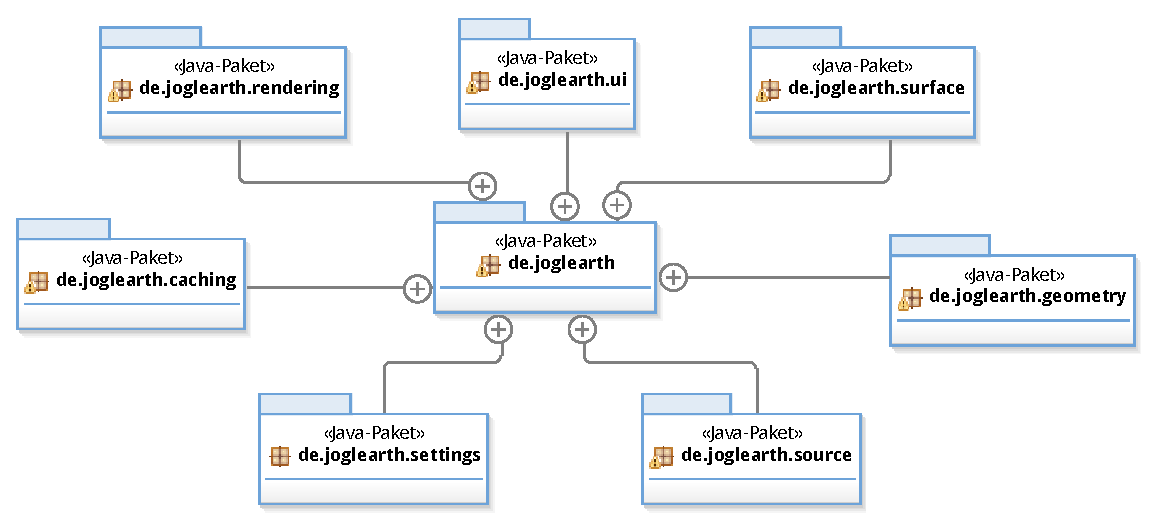
\includegraphics[scale=0.55]{Pakete.eps}
\end{center}
\end{figure}

\begin{itemize}
\item \textbf{\sffamily de.joglearth} ist der Container für alle anderen Packages und enthält die Hauptklasse \textit{JoglEarth}.
\begin{itemize}
\item \textbf{\sffamily de.joglearth.caching} stellt die Caching-Funktionalität bereit.
\item \textbf{\sffamily de.joglearth.geometry} beinhaltet Klassen für die geometrischen Ansichts- und Sichtbarkeitsberechnungen sowie die mathematische Beschreibung der Darstellungsmodelle.
\item \textbf{\sffamily de.joglearth.rendering} enthält Klassen zur Umsetzung des mathematischen Modells in eine 3D-Darstellung mit OpenGL.
\item \textbf{\sffamily de.joglearth.settings} ist für die Verwaltung von Benutzereinstellungen und Benachrichtigung bei deren Änderung zuständig.
\item \textbf{\sffamily de.joglearth.source} beinhaltet Klassen zum synchronen und asynchronen Zugriff auf externe Daten.
\item \textbf{\sffamily de.joglearth.surface} enthält Komponenten zur Verwaltung von Objekten und Eigenschaften der Erdoberfläche wie dem Kartenmaterial, dem Höhenprofil und der Overlays.
\item \textbf{\sffamily de.joglearth.ui} fasst Klassen der grafischen Benutzeroberfläche zusammen.
\end{itemize}
\end{itemize}

\newpage

\section{Interfaces, Klassen und Enumerations}

Im Folgenden werden UML-Diagramme für die Elemente der einzelnen Packages gezeigt.

\vspace{5mm}

\begin{figure}[!htb]
	\centering
		\begin{minipage}[c]{3cm}
        \centering
			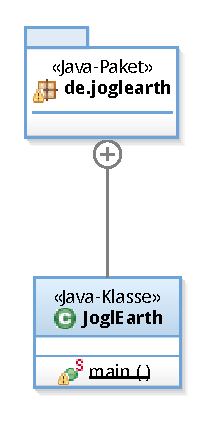
\includegraphics[scale=0.55]{de_joglearth.eps}
        \end{minipage}
        \hspace{2cm}
        \begin{minipage}[c]{6cm}
        \centering
			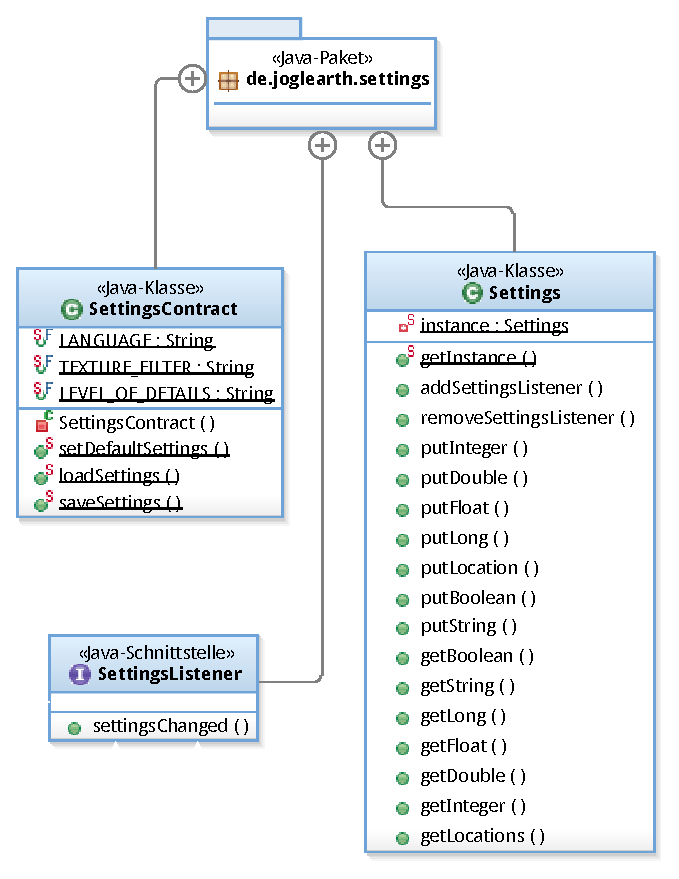
\includegraphics[scale=0.55]{de_joglearth_settings.eps}
        \end{minipage}
        \caption{Packages de.joglearth und de.joglearth.settings}
\end{figure}

\vspace{5mm}

\begin{figure}[!htb]
\begin{center}
	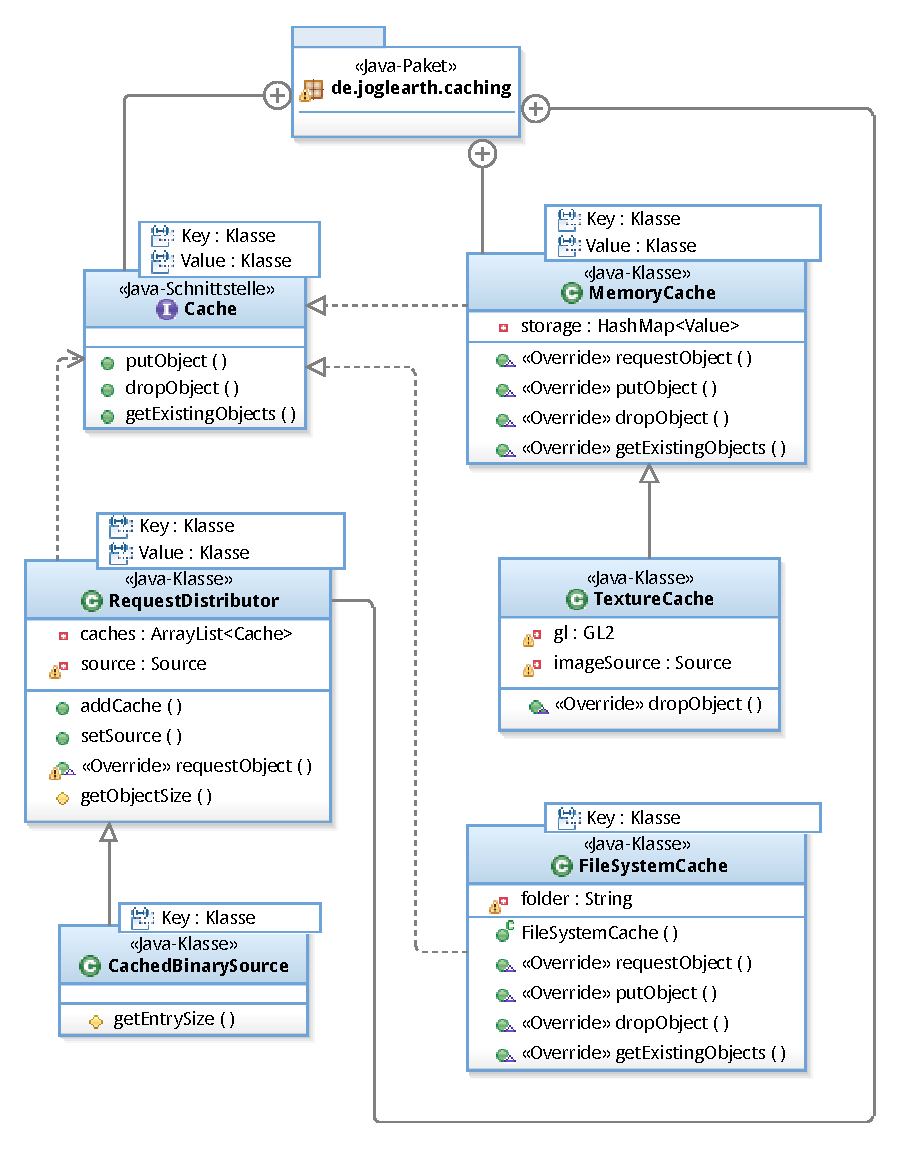
\includegraphics[scale=0.55]{de_joglearth_caching.eps}
\end{center}
\caption{Das Package de.joglearth.caching}
\end{figure}


\begin{figure}[!htb]
\begin{center}
	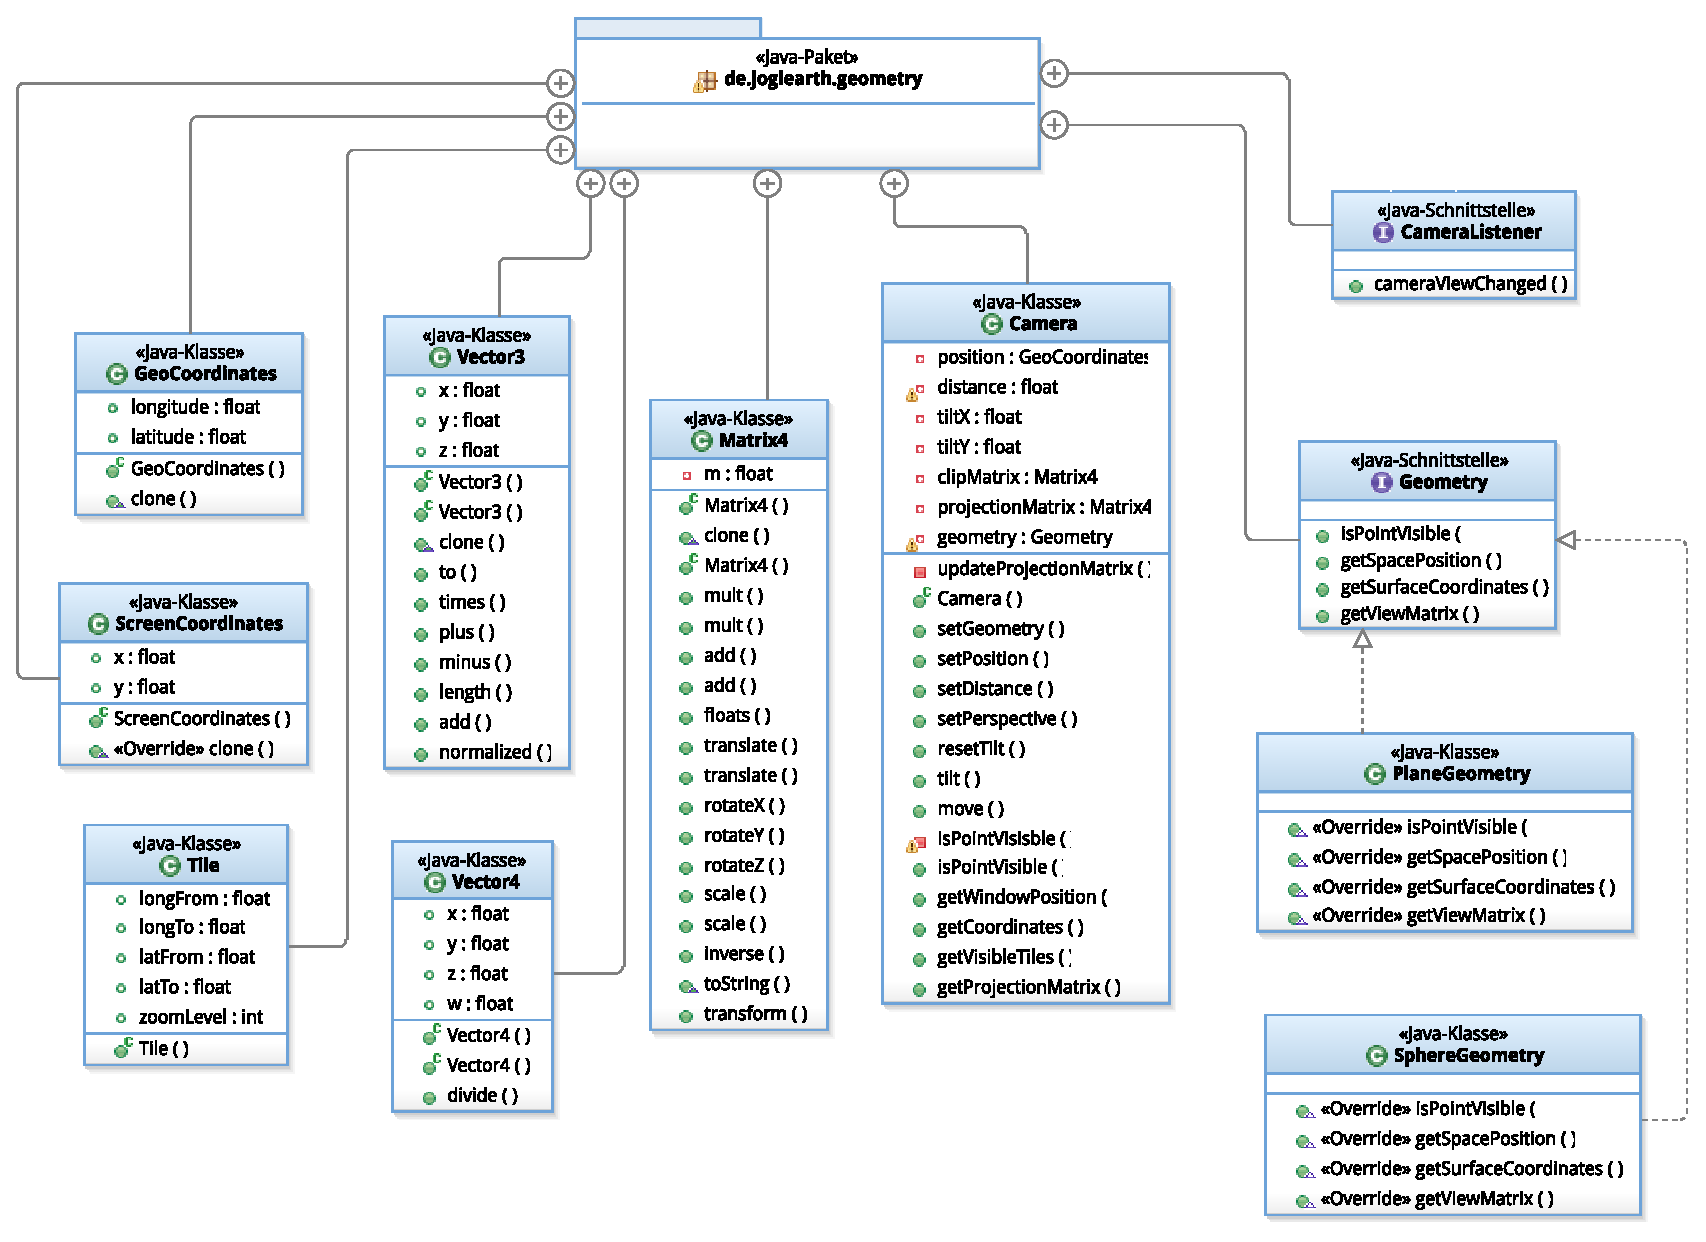
\includegraphics[scale=0.55]{de_joglearth_geometry.eps}
\end{center}
\caption{Das Package de.joglearth.geometry}
\end{figure}

\begin{figure}[!htb]
\begin{center}
	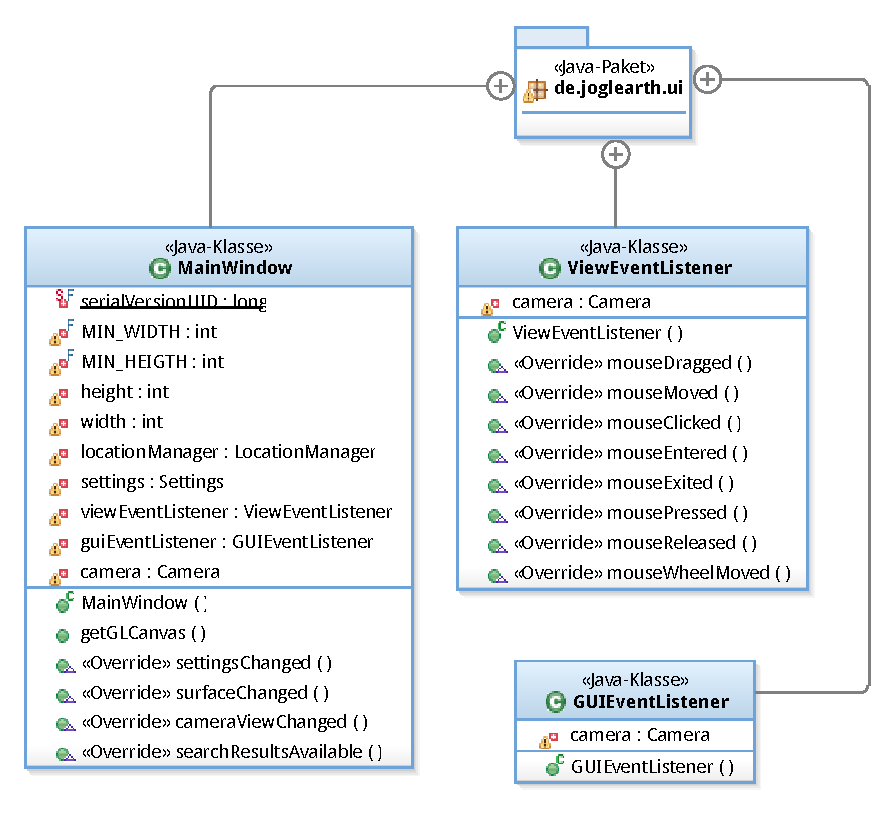
\includegraphics[scale=0.55]{de_joglearth_ui.eps}
\end{center}
\caption{Das Package de.joglearth.ui}
\end{figure}

\begin{figure}[!htb]
\begin{center}
	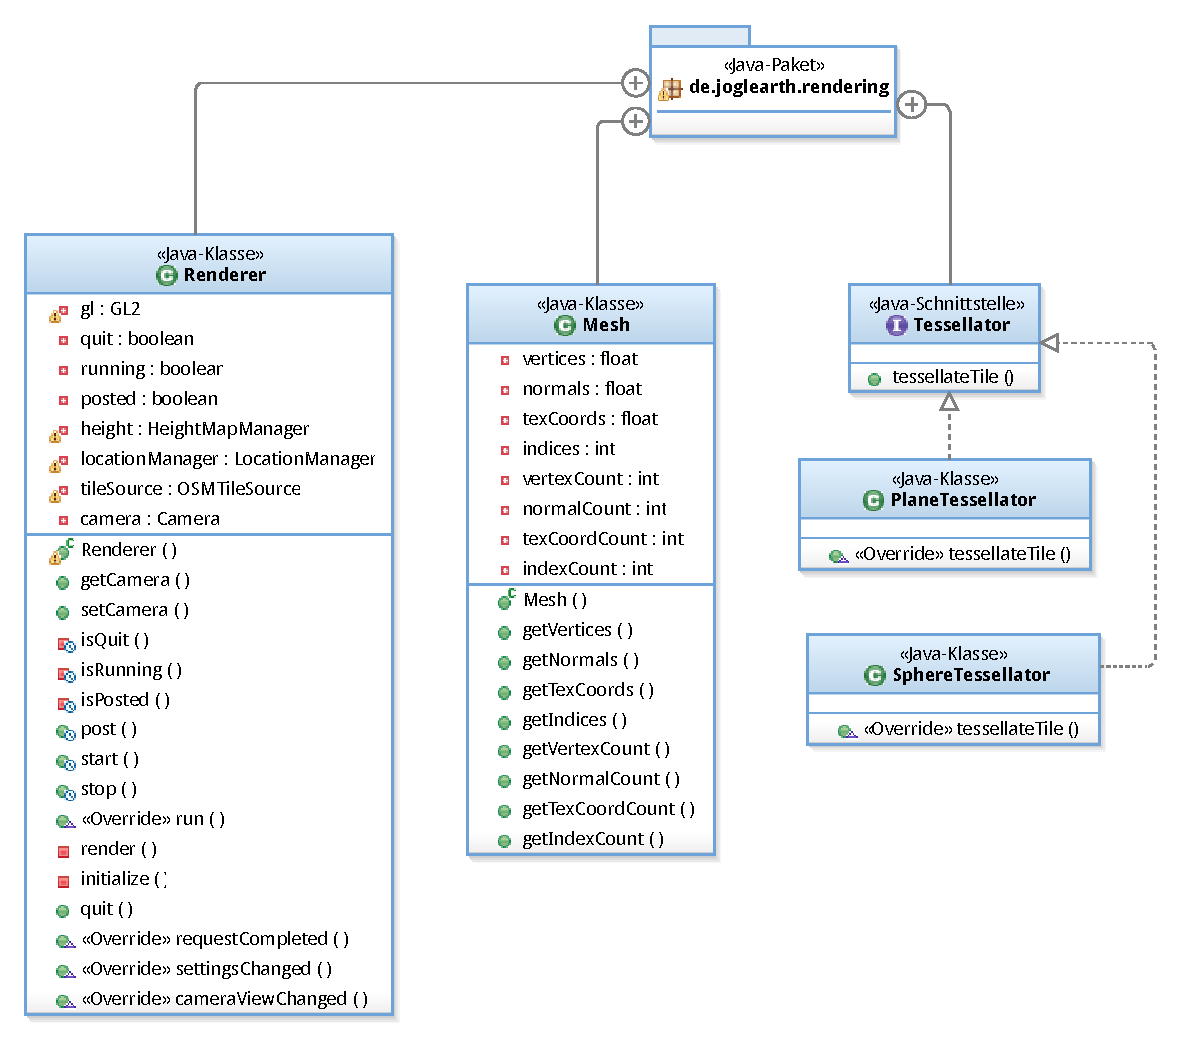
\includegraphics[scale=0.55]{de_joglearth_rendering.eps}
\end{center}
\caption{Das Package de.joglearth.rendering}
\end{figure}

\begin{figure}[!htb]
\begin{center}
	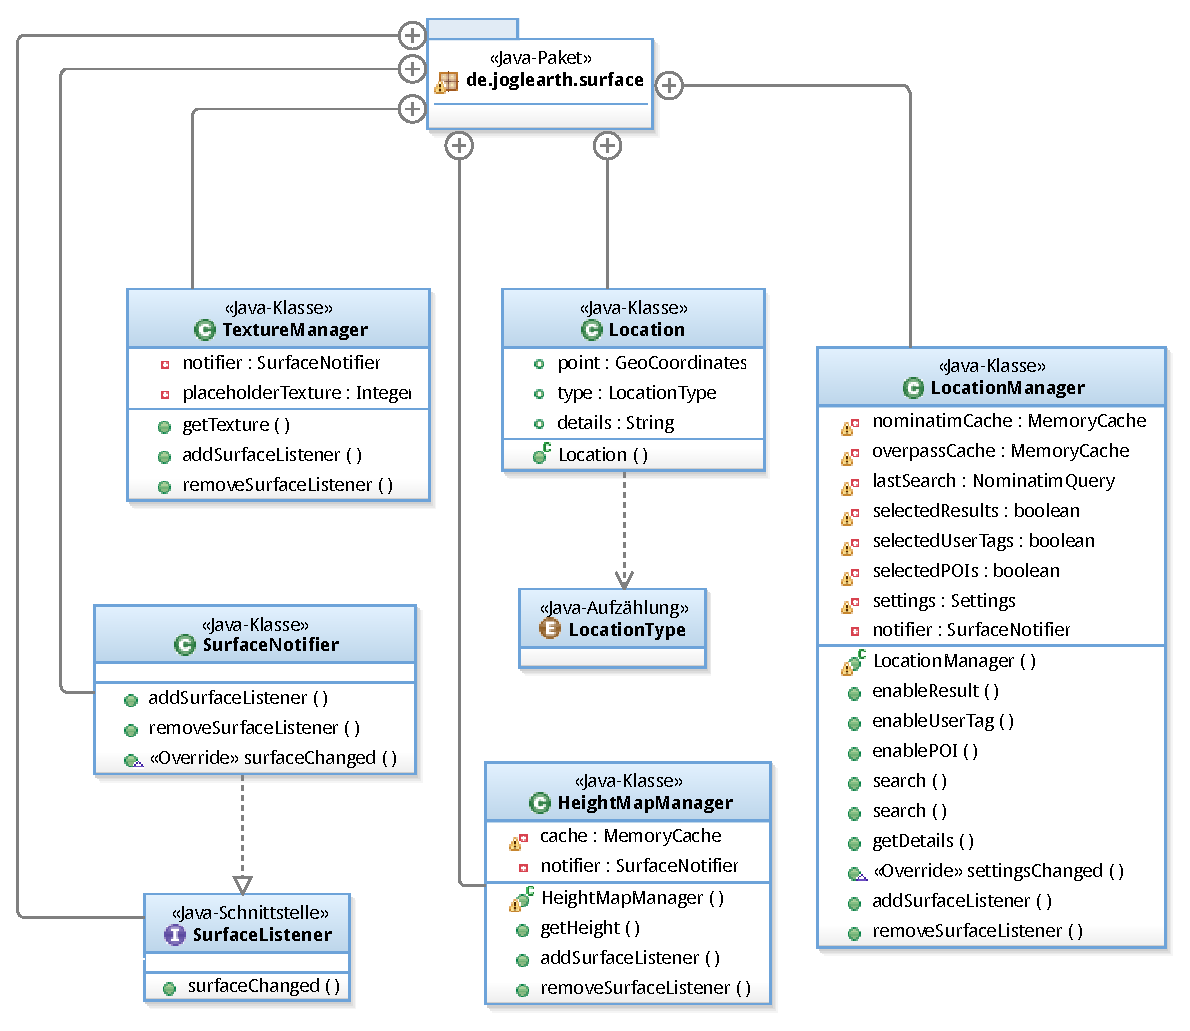
\includegraphics[scale=0.55]{de_joglearth_surface.eps}
\end{center}
\caption{Das Package de.joglearth.surface}
\end{figure}


\begin{figure}[!htb]
\begin{center}
	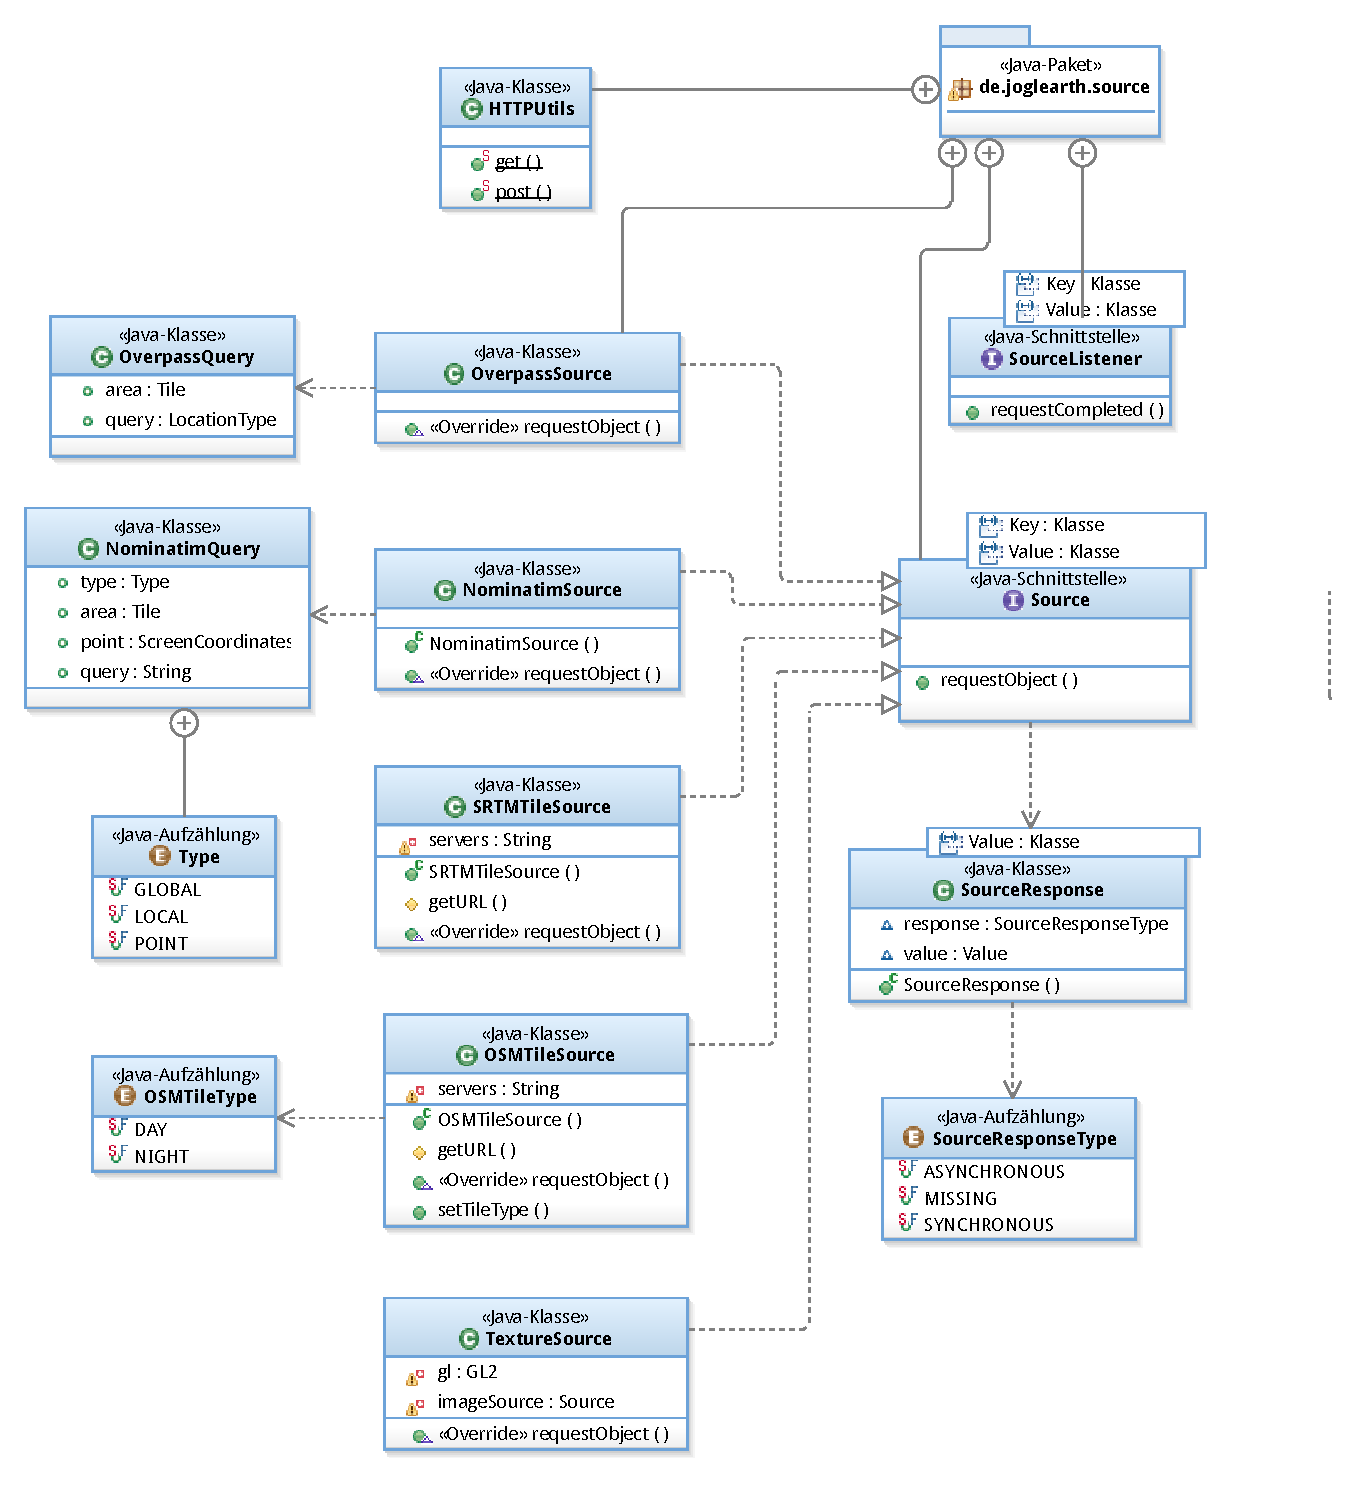
\includegraphics[scale=0.55]{de_joglearth_source.eps}
\end{center}
\caption{Das Package de.joglearth.source}
\end{figure}



\chapter{Beschreibung der Interfaces}

\section{Package de.joglearth.caching}
\subsection*{Cache}
\begin{lstlisting}
interface Cache<Key, Value>
extends Source<Key, Value>
\end{lstlisting}
Bildet die Schnittstelle für einen Cache, der Methoden zum Hinzufügen, Abfragen und Löschen von Daten bietet.\\


\vspace{5mm}
\section{Package de.joglearth.geometry}
\subsection*{Geometry}
\begin{lstlisting}
interface Geometry
\end{lstlisting}
Abstrahiert die Sichtbarkeitsberechnungen verschiedener Oberflächenmodelle, wie eines Globus oder einer Kartenebene.\\

\vspace{5mm}
\subsection*{CameraListener}
\begin{lstlisting}
interface CameraListener
\end{lstlisting}
Interface für Klassen, die Events beim Ändern der Kameraeinstellungen .\\


\vspace{5mm}
\section{Package de.joglearth.rendering}
\subsection*{Tessellator}
\begin{lstlisting}
interface Tessellator
\end{lstlisting}
Bietet eine gemeinsame Schnittstelle für das Erzeugen von dreidimensionalen Kacheln verschiedener Modelle.\\


\vspace{5mm}
\section{Package de.joglearth.settings}
\subsection*{SettingsListener}
\begin{lstlisting}
interface SettingsListener
\end{lstlisting}
Eine Implementierung des \textit{SettingsListeners} kann über Änderungen der \textit{Settings} benachrichtigt werden.\\


\vspace{5mm}
\section{Package de.joglearth.source}
\subsection*{Source}
\begin{lstlisting}
interface Source<Key, Value>
\end{lstlisting}
Ist in der Lage, über einen \texttt{Key} identifizierte Objekte synchron oder asynchron zu beschaffen.\\

\vspace{5mm}
\subsection*{SourceListener}
\begin{lstlisting}
interface SourceListener<Key, Value>
\end{lstlisting}
Eine Implementierung dies Interfaces kann asynchrone Antworten einer \textit{Source} entgegen nehmen.\\


\vspace{5mm}
\section{Package de.joglearth.surface}
\subsection*{SurfaceListener}
\begin{lstlisting}
interface SurfaceListener
\end{lstlisting}
Eine Implementierung dieses Interfaces kann über Änderung der Darstellung einzelner Kartenkacheln benachrichtigt werden.\\

\vspace{5mm}
\subsection*{LocationListener}
\begin{lstlisting}
interface LocationListener
\end{lstlisting}
Eine Implementierung dieses Interfaces nimmt asynchrone Antworten des \textit{LocationManagers}, wie geladene Suchergebnisse, entgegen.\\




\chapter{Klassenbeschreibung}
\section{Package de.joglearth}
\begin{lstlisting}
final class JoglEarth
\end{lstlisting}
Die Klasse \textit{JoglEarth} implementiert die Main-Methode zum Starten des Programms.\\

\vspace{5mm}
\section{Package de.joglearth.caching}
\subsection*{CachedBinarySource}
\begin{lstlisting}
class CachedBinarySource<Key>
extends RequestDistributor<Key, byte[]>
\end{lstlisting}
Erweitert den \textit{RequestDistributor} um die Möglichkeit den Cache nach Größe statt nach Anzahl der Einträge zu begrenzen.\\

\vspace{5mm}
\subsection*{RequestDistributor}
\begin{lstlisting}
class RequestDistributor<Key, Value>
implements Source<Key, Value>
\end{lstlisting}
Lädt Daten aus einer \textit{Source}, verwaltet diese in Caches und ist für deren Verdrängung verantwortlich.\\

\vspace{5mm}
\subsection*{FileSystemCache}
\begin{lstlisting}
class FileSystemCache<Key>
implements Cache<Key, byte[]>
\end{lstlisting}
Ein \textit{FileSystemCache} speichert Daten im Dateisystem zwischen.\\

\vspace{5mm}
\subsection*{MemoryCache}
\begin{lstlisting}
class MemoryCache<Key, Value>
implements Cache<Key, Value>
\end{lstlisting}
Ein \textit{MemoryCache} speichert Daten im Arbeitsspeicher ähnlich einer \textit{HashMap} zwischen.\\

\newpage
\vspace{5mm}
\subsection*{TextureCache}
\begin{lstlisting}
class TextureCache
extends MemoryCache<Tile, Integer>
\end{lstlisting}
Ein \textit{TextureCache} verwaltet in OpenGL geladene Texturen.


\vspace{5mm}
\section{Package de.joglearth.geometry}
\subsection*{Camera}
\begin{lstlisting}
class Camera
\end{lstlisting}
Berechnet die Projektionsmatrix für den Rendervorgang, bestimmt die Sichtbarkeit von 3D-Objekten im Ansichtsfenster und rechnet zwischen Bildschirm- und Raumkoordinaten um.\\
Enthält eine Methode zum Setzen einer \textit{Geometry} für die Unterscheidung zwischen sphärischen und planaren Bewegungsberechnungen.\\

\vspace{5mm}
\subsection*{GeoCoordinates}
\begin{lstlisting}
class GeoCoordinates
implements Cloneable
\end{lstlisting}
Speichert Längen- und Breitengrad eines Punktes auf der Erdoberfläche.\\

\vspace{5mm}
\subsection*{Matrix4}
\begin{lstlisting}
class Matrix4
implements Cloneable
\end{lstlisting}
Hält eine 4x4-Matrix, die Operationen zum Rotieren, Verschieben und Skalieren, sowie eine Funktion zum transformieren eines dreidimensionalen Vektors anbietet. Sie wird zum von der Kamera intern zum Bestimmen der Projektionsmatrix und der Sichtbarkeit von Objekten verwendet.\\

\vspace{5mm}
\subsection*{PlaneGeometry}
\begin{lstlisting}
class PlaneGeometry
implements Geometry
\end{lstlisting}
Implementiert das \textit{Geometry}-Interface für räumliche Berechnungen auf einer Ebene.\\

\vspace{5mm}
\subsection*{ScreenCoordinates}
\begin{lstlisting}
class ScreenCoordinates
implements Cloneable
\end{lstlisting}
Stellt einen Punkt auf der Bildschirmebene in relativen Koodrinaten zwischen 0 und 1 dar.\\

\newpage
\vspace{5mm}
\subsection*{SphereGeometry}
\begin{lstlisting}
class SphereGeometry
implements Geometry
\end{lstlisting}
Implementiert das \textit{Geometry}-Interface für räumliche Berechnungen auf der Kugeloberfläche.\\

\vspace{5mm}
\subsection*{Tile}
\begin{lstlisting}
class Tile 
implements Cloneable
\end{lstlisting}
Speichert Längen- und Breitengradgrenzen sowie das Zoomlevel, über das sich eine Kartenkachel nach dem OpenStreetMap-Format identifizieren lässt.\\

\vspace{5mm}
\subsection*{Vector3}
\begin{lstlisting}
class Vector3
implements Cloneable
\end{lstlisting}
Ein 3-dimensionaler Vektor. Repräsentiert üblicherweise Raumkoordinaten.\\

\vspace{5mm}
\subsection*{Vector4}
\begin{lstlisting}
class Vector4
implements Cloneable
\end{lstlisting}
Ein 4-dimensionaler Vektor für homogene Koordinaten. Instanzen dieser Klasse werden benötigt, wenn zwischen 3D-Perspektiven umgerechnet werden soll.\\





\vspace{5mm}
\section{Package de.joglearth.rendering}
\subsection*{Mesh}
\begin{lstlisting}
class Mesh
\end{lstlisting}
Speichert Rohdaten eines 3D-Modells wie seine Vertices, Normalen, und Texturkoordinaten. Meshes werden unter Anderem von Tessellatoren generiert und vom \textit{Renderer} an OpenGL übergeben.\\

\vspace{5mm}
\subsection*{PlaneTessellator}
\begin{lstlisting}
class PlaneTessellator
implements Tessellator
\end{lstlisting}
Generiert Kachelmeshes in der Ebene.\\

\newpage
\vspace{5mm}
\subsection*{Renderer}
\begin{lstlisting}
class Renderer
implements SourceListener<Tile, Integer>, Runnable, CameraListener,
           SettingsListener
\end{lstlisting}
Ist für das Zeichnen einzelner Frames und die zeitliche Steuerung während Animationen verantwortlich. Rendert entweder Einzelbilder als Reaktion auf eine Aktualisierung über den \textit{SourceListener}, \textit{CameraListener} oder \textit{SettingsListener} oder eine kontinuierliche Bildfolge während Animationsvorgängen.\\
Enthält neben der start()-Methode eine weitere Methode post() mit der er zum einmaligen rendern angestoßen wird.\\
\vspace{5mm}
\subsection*{SphereTessellator}
\begin{lstlisting}
class SphereTessellator
implements Tessellator
\end{lstlisting}
Generiert Kachelmeshes auf der Globusoberfläche.\\




\vspace{5mm}
\section{Package de.joglearth.settings}
\subsection*{Settings}
\begin{lstlisting}
class Settings
\end{lstlisting}
Verwaltet alle erforderlichen Einstellungen sowie die vom Benutzer markierten Punkte aus der Datei \texttt{settings.xml}. Die Einstellungen werden gekapselt und anderen Klassen zugänglich gemacht, außerdem können sich andere Klassen als Beobachter (\textit{Observer}) registrieren um über Einstellungsänderungen benachrichtigt zu werden.\\

\vspace{5mm}
\subsection*{SettingsContract}
\begin{lstlisting}
final class SettingsContract
\end{lstlisting}
Speichern und laden von Settings. Verwaltet die IDs der verschiedenen Settings.\\



\vspace{5mm}
\section{Package de.joglearth.source}
\subsection*{HTTPUtils}
\begin{lstlisting}
final class HTTPUtils
\end{lstlisting}
Stellt statische Funktionen für einfache GET- und POST- Abfragen via HTTP zur Verfügung.\\

\vspace{5mm}
\subsection*{NominatimQuery}
\begin{lstlisting}
class NominatimQuery
\end{lstlisting}
Drückt eine Suchanfrage an Nominatim aus. Dies kann die Suche nach Details zu einem bestimmten Punkt oder nach einem Ort sein.\\

\vspace{5mm}
\subsection*{NominatimSource}
\begin{lstlisting}
class NominatimSource
implements Source<NominatimQuery, Location[]>
\end{lstlisting}
\textit{NominatimSource} beschafft Antworten auf Suchanfragen nach Orten und Punktinformationen (\textit{NominatemQuery}) und bereitet sie für den \textit{LocationManager} auf. Dabei greift sie auf \textit{HTTPUtils} zu.\\

\vspace{5mm}
\subsection*{OSMTileSource}
\begin{lstlisting}
class OSMTileSource
implements Source<Tile, byte[]>
\end{lstlisting}
Die \textit{OSMTileSource} lädt anhand von Koordinaten (u. U. komprimierte) Kacheltexturen per HTTP von OpenStreetMap-Servern. Dabei macht sie von \textit{HTTPUtils} Gebrauch.\\

\vspace{5mm}
\subsection*{OverpassQuery}
\begin{lstlisting}
class OverpassQuery
\end{lstlisting}
Drückt eine Suchanfrage an die OverpassAPI aus. Eine solche Suche liefert für gewöhnlich POIs und Städtenamen im Sichtfeld zurück. Die Anfrage enthält dazu die zu durchsuchende Umgebung.\\

\vspace{5mm}
\subsection*{OverpassSource}
\begin{lstlisting}
class OverpassSource
implements Source<OverpassQuery, Location[]>
\end{lstlisting}
\textit{OverpassSource} beschafft die Details lokaler POIs und Städtenamen (\textit{OverpassQuery}) und bereitet sie für die Verwaltung durch den \textit{LocationManager} vor.\\

\vspace{5mm}
\subsection*{SourceResponse}
\begin{lstlisting}
class SourceResponse<Value>
\end{lstlisting}
Rückgabetyp der \textit{Source} inkl. Informationen über die Art der Nachlieferung.\\

\vspace{5mm}
\subsection*{SRTMTileSource}
\begin{lstlisting}
class SRTMTileSource
implements Source<Tile, byte[]>
\end{lstlisting}
Die \textit{SRTMTileSource} lädt anhand von Indizes Höhenprofil-Kacheln von NASA-SRTM-Servern. Dabei macht sie von \textit{HTTPUtils} Gebrauch.\\

\newpage
\vspace{5mm}
\subsection*{TextureSource}
\begin{lstlisting}
class TextureSource
implements Source<Tile, Integer>
\end{lstlisting}
Lädt die Texturen in OpenGL.\\



\vspace{5mm}
\section{Package de.joglearth.surface}
\subsection*{HeightMapManager}
\begin{lstlisting}
class HeightMapManager
implements SettingsListener
\end{lstlisting}
Interpoliert Höheninformationen für Punkte der Karte aus SRTM-Höhendaten. Wird von \textit{Tessellator}en verwendet, um Kartenoberflächen mit dem Höhenprofil zu generieren.\\

\vspace{5mm}
\subsection*{Location}
\begin{lstlisting}
class Location
implements Cloneable
\end{lstlisting}
Speichert Längen- und Breitengradkoordinaten mit Details zu einem Punkt ab. Wird vom \textit{LocationManager} benutzt, um alle Arten von Punkten auf der Karte zu verwalten.\\

\vspace{5mm}
\subsection*{LocationManager}
\begin{lstlisting}
class LocationManager
implements SettingsListener
\end{lstlisting}
Verwaltet die Sichtbarkeit von besonderen Punkten im Ansichtsfenster und der GUI. Er besorgt außerdem Suchergebnisse über den \textit{NominatimSource} und Benutzermarkierungen aus den \textit{Settings}.\\

\vspace{5mm}
\subsection*{TextureManager}
\begin{lstlisting}
class TextureManager
\end{lstlisting}
Bearbeitet Texturanfrage vom \textit{Renderer}. Lädt die Texturen aus einem \textit{RequestDistributor} die auf einem \textit{TextureSource} und einem \textit{TextureCache} zurückgreift.\\




\vspace{5mm}
\section{Package de.joglearth.ui}
\subsection*{GUI}
\begin{lstlisting}
class GUI
extends JFrame
implements SurfaceListener, CameraListener, SettingsListener
\end{lstlisting}
Die Klasse \textit{GUI} erbt von JFrame und stellt die gesamte grafische Bedienoberfläche dar. Pro Sitzung darf lediglich eine Instanz der \textit{GUI} existieren.\\

\vspace{5mm}
\subsection*{GUIEventListener}
\begin{lstlisting}
class GUIEventListener
\end{lstlisting}
Reagiert auf Ereignisse der Swing-Elemente der GUI; d.h. auf alle Benutzereingaben die außerhalb des Ansichtsfensters stattfinden. Verändert unter Umständen Werte von \textit{Settings} oder gibt Ereignisse an den Renderer oder andere Komponenten über den \textit{UpdateListener}-Mechanismus weiter.\\

\vspace{5mm}
\subsection*{ViewEventListener}
\begin{lstlisting}
class ViewEventListener
implements /* zum Beispiel */ MouseWheelListener, MouseListener, MouseMotionListener
\end{lstlisting}
Reagiert auf Benutzereingaben im Ansichtsfenster wie Tastendrücke, Scrollen und Ziehen mit der Maus. Die Klasse benachrichtigt andere Komponenten, wie die \textit{Camera}, über Veränderungen der Ansicht.\\




\chapter{Beschreibung der Enumerations}
\section*{Package de.joglearth.source}

\subsection*{NominatimQuery.Type}
\begin{tabular}{p{4cm} p{11cm}}
\textit{GLOBAL} & Globale Suche nach Punkten \\
\textit{LOCAL} & Suche nach Punkten im Sichtbereich \\
\textit{POINT} & Alle verfügbaren Informationen zu einem bestimmten Punkt \\
\end{tabular}

\vspace{5mm}
\subsection*{OSMTileType}
Stellt eine Unterscheidung der verschiedenen Kartenmaterialien dar.

\vspace{5mm}
\subsection*{SourceResponseType}
\begin{tabular}{p{4cm} p{11cm}}
\textit{ASYNCHRONOUS} & Das Ergebnis der Anfrage der \textit{SourceResponse} wird asynchron über \textit{requestCompleted} rückgemeldet\\
\textit{MISSING} & Die \textit{Source} ist nicht in der Lage das angeforderte Objekt zu beschaffen\\
\textit{SYNCHRONOUS} & Das Ergebnis der Anfrage ist lokal in einem \textit{Cache} verfügbar und wird unmittelbar rückgeliefert \\
\end{tabular}


\vspace{5mm}
\section*{Package de.joglearth.surface}
\subsection*{LocationType}
Stellt die unterschiedlichen Typen von Overlays wie POIs, Städtenamen oder markierte Punkte dar.



\chapter{Sequenzdiagramme}

\section{Lokale Suche nach einem Begriff}
Dieses Sequenzdiagramm zeigt, wie eine lokale Suche nach einem Begriff vom \textit{LocationManager} entgegengenommen und über die \textit{NominatimSource} beantwortet wird.\\[3mm]
Eine größere Version des Diagramms findet sich im Anhang (\textref Abbildung 9.1).

\vspace*{5mm}
\begin{figure}[h]
\begin{center}
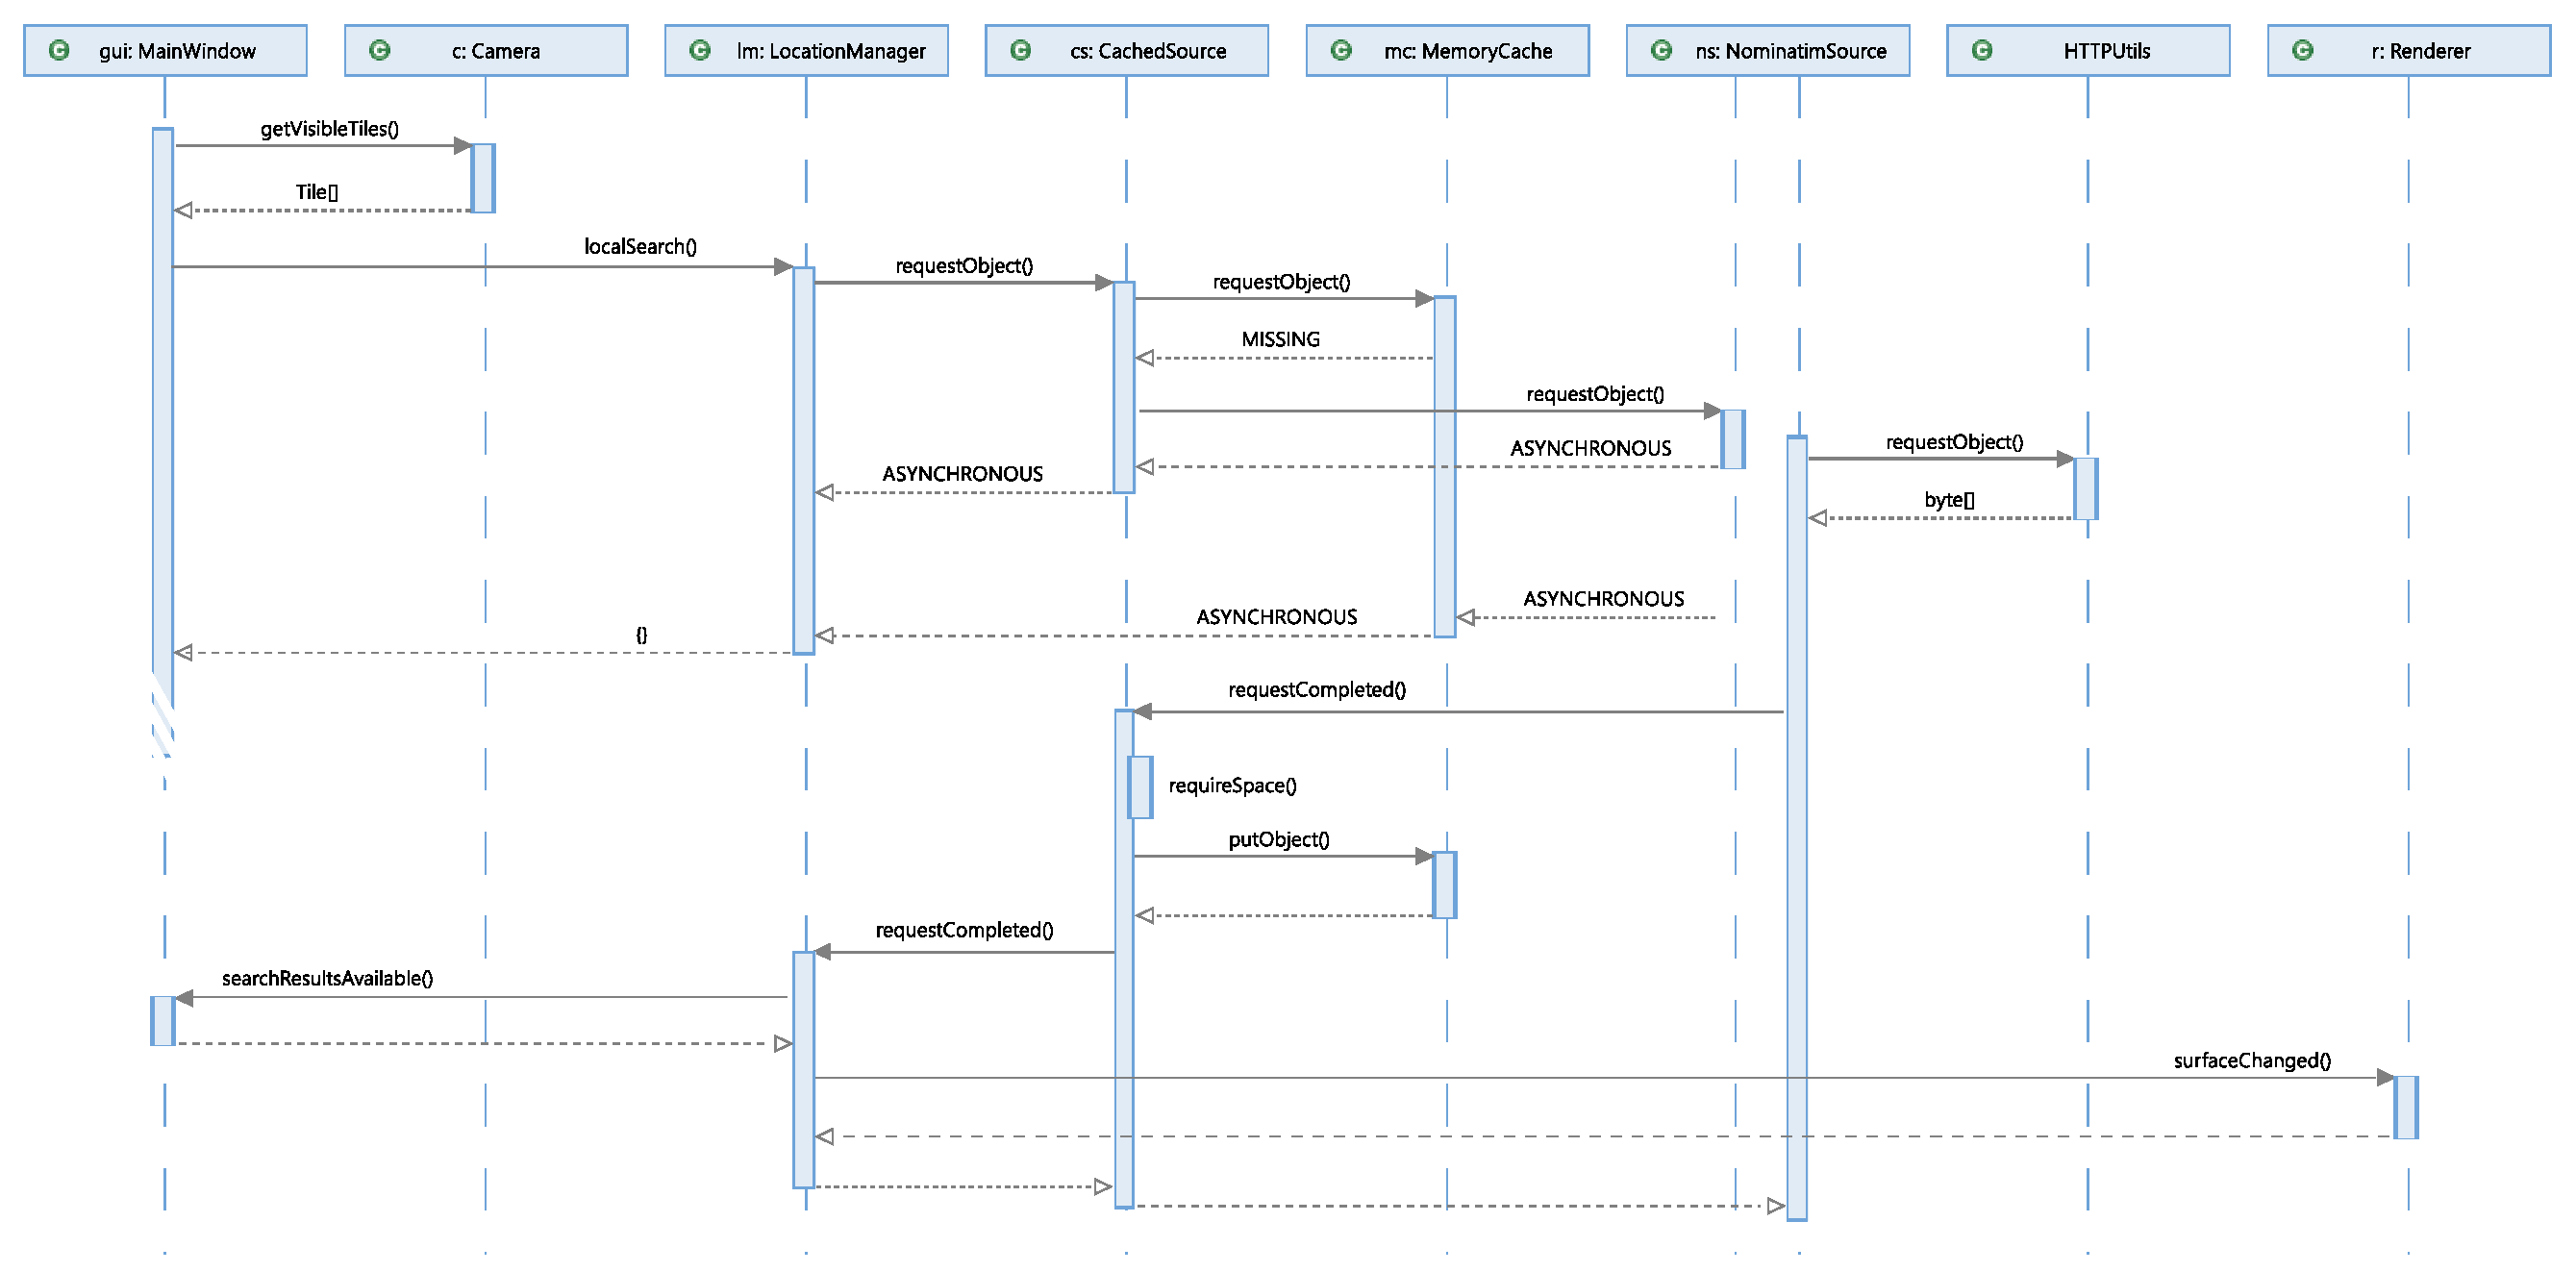
\includegraphics[scale=0.28]{sequenz-search.eps}
\caption{Lokale Suche nach einem Begriff}
\end{center}
\end{figure}

\begin{itemize}
\item Die GUI übergibt dem \textit{LocationManager} einen Suchbegriff und die sichtbaren Kacheln, die er von der Kamera erhalten hat.
\item Dieser fordert von seinem \textit{RequestDistributor} die Suchergebnisse zu dieser Anfrage an, der wegen des Fehlens des Ergebnisses in seinem \textit{MemoryCache} bei der \textit{NominatimSource} eine Anfrage startet. 
\item Da eine Anfrage über das Internet zeitaufwändig ist, kehrt sie und damit der \textit{RequestDistributor} mit der Notiz zurück, dass eine asynchrone Antwort folgt. Die GUI erhält daher zuerst ein leeres Ergebnis.
\item Wurde die Anfrage beantwortet, benachrichtigt die \textit{NominatimSource} den \textit{RequestDistributor}, der die Antwort in seinen \textit{MemoryCache} legt und seinerseits den \textit{LocationManager} benachrichtigt.
\item Der GUI, die ein \textit{LocationListener} ist, wird mitgeteilt, dass die Suchergebnisse jetzt verfügbar sind.
\end{itemize}
\newpage


\section{Laden einer lokal noch nicht vorhandenen Kachel}

In diesem Sequenzdiagramm wird dargestellt, wie die Anfrage nach einer Texturkachel über die verschiedenen Cacheebenen propagiert und schließlich asynchron beantwortet wird.\\[3mm]
Eine größere Version des Diagramms findet sich im Anhang (\textref Abbildung 9.2).

\vspace*{5mm}
\begin{figure}[h]
\begin{center}
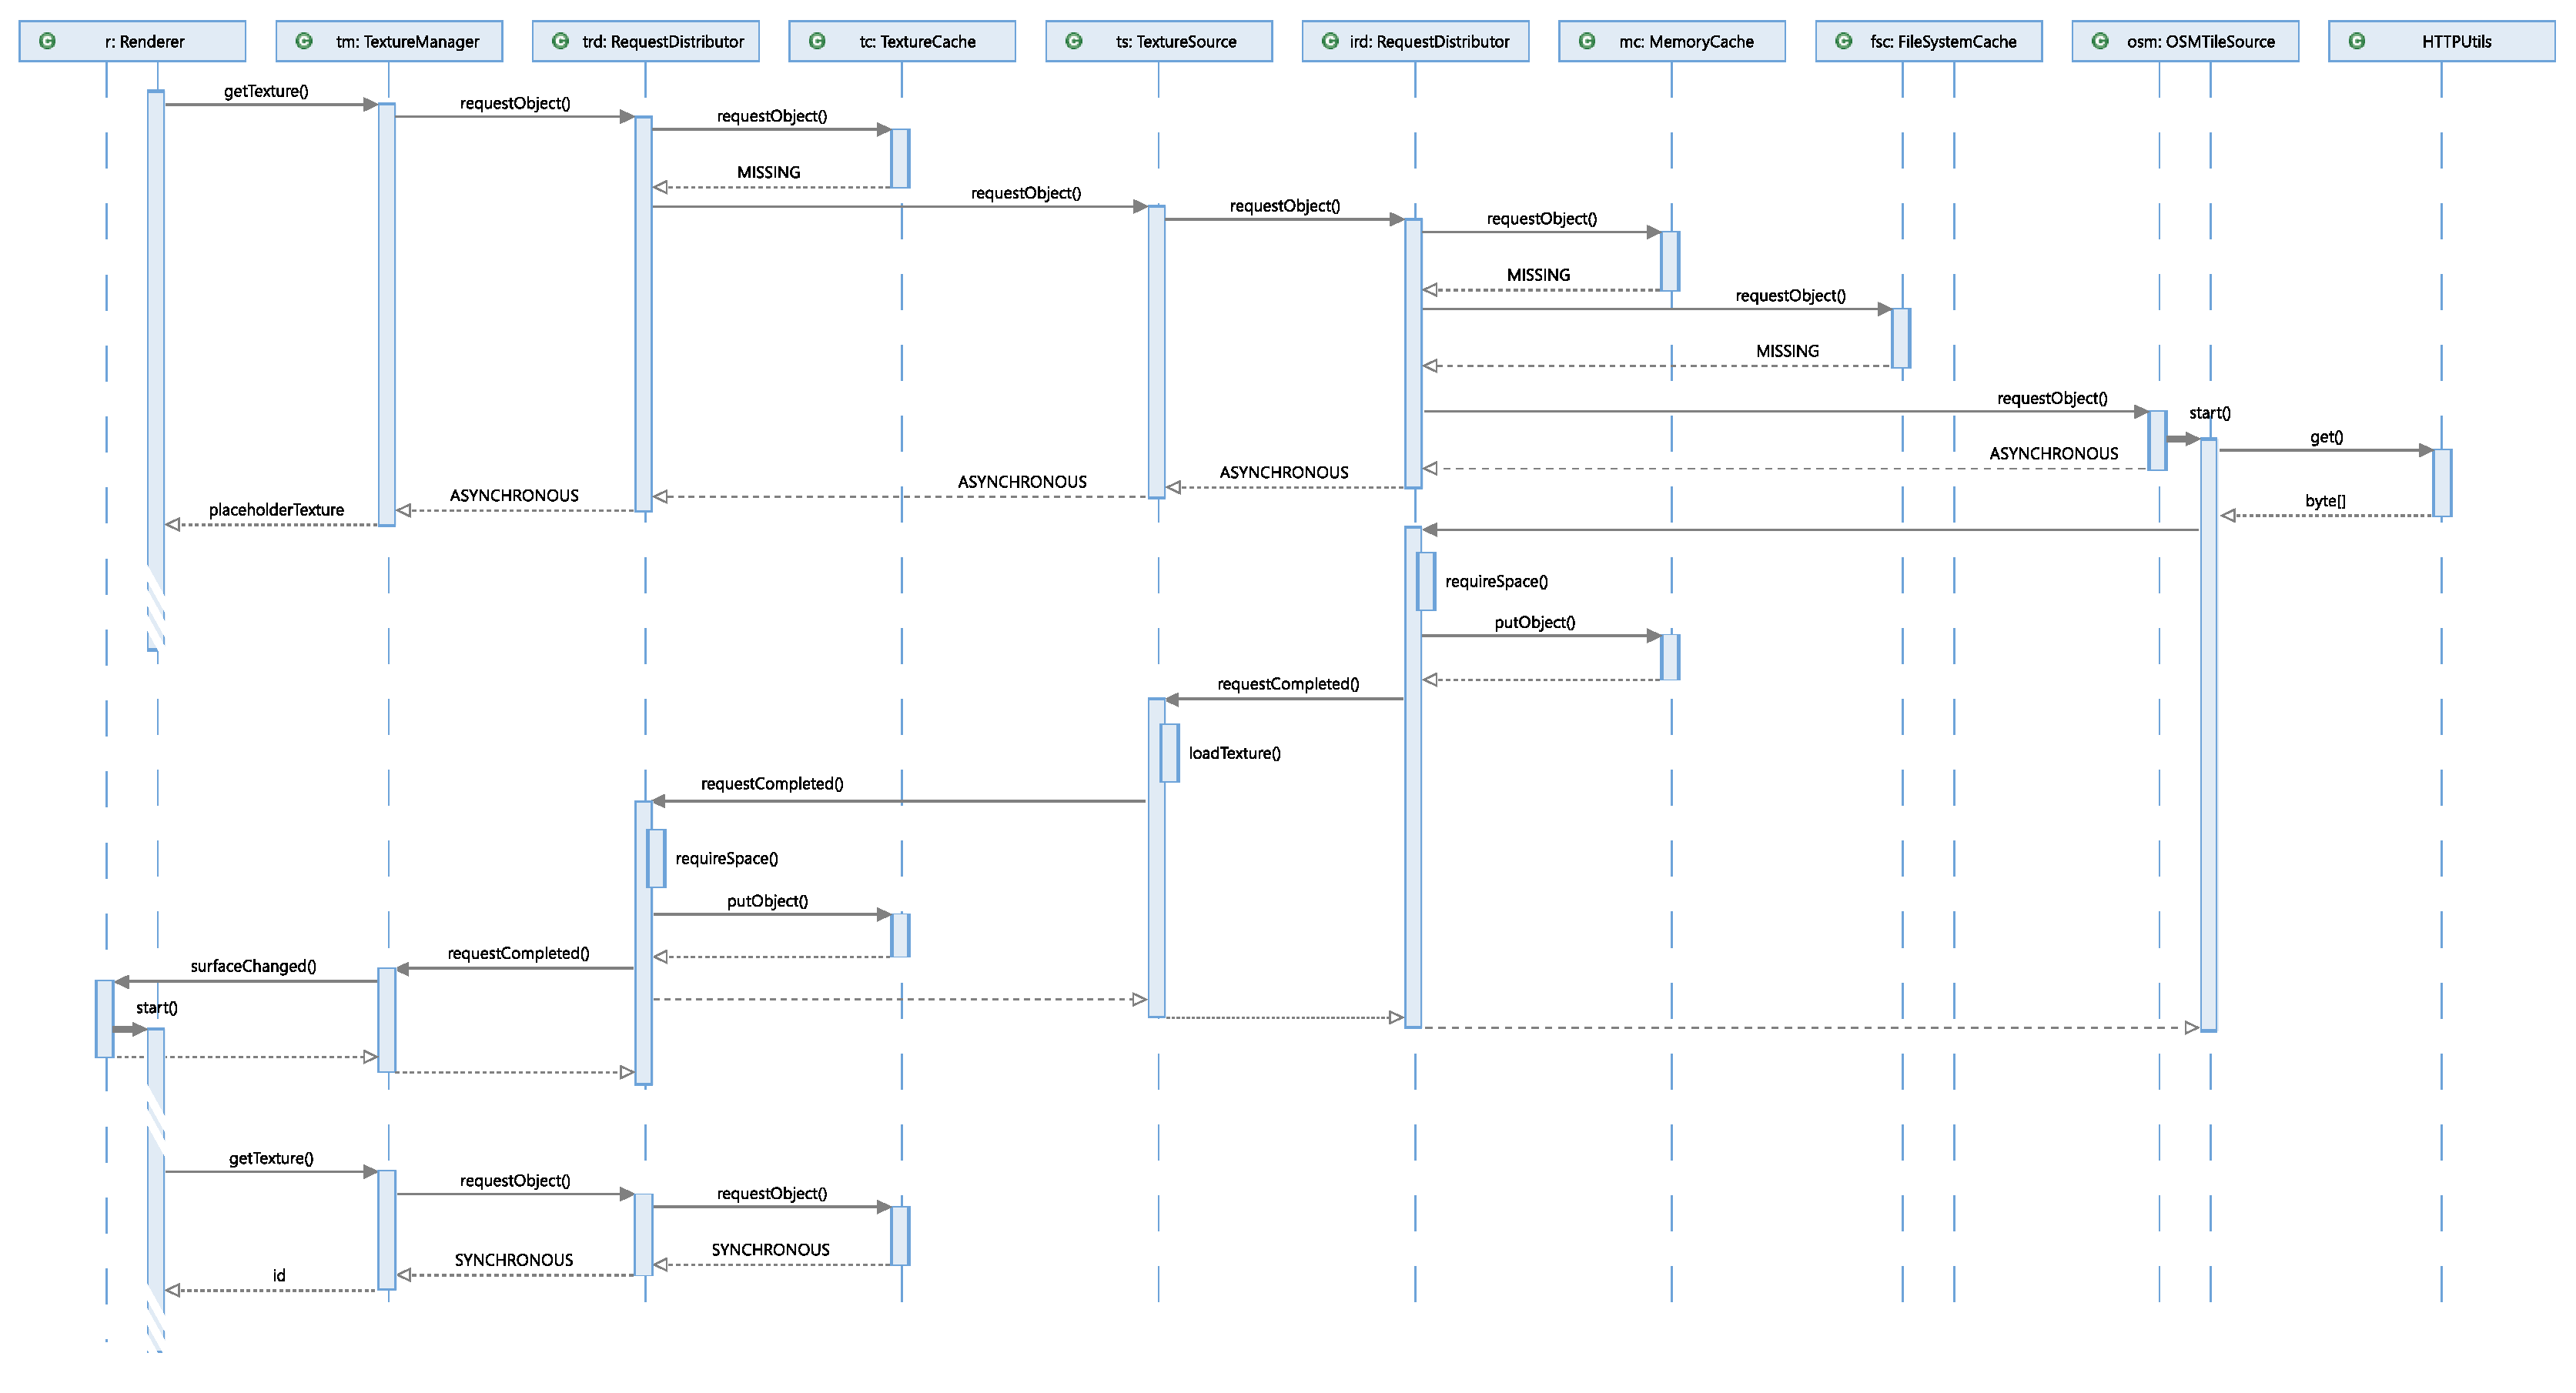
\includegraphics[scale=0.28]{sequenz-osmtile.eps}
\caption{Laden einer lokal noch nicht vorhandenen Kachel}
\end{center}
\end{figure}

\begin{itemize}
\item Der \textit{Renderer} fragt den \textit{TextureManager} nach der Textur die gerendert werden soll.
\item Dieser fordert von seinem \textit{RequestDistributor} die Suchergebnisse zu dieser Anfrage an, der wegen des Fehlens des Ergebnisses in seinem \textit{TextureCache} bei der \textit{TextureSource} eine Anfrage startet.
\item In unserem Beispiel ist die Textur noch nicht im \textit{TextureCache} vorhanden. Deswegen leitet der \textit{RequestDistributor} die Anfrage an die \textit{TextureSource} weiter.
\item Die \textit{TextureSource} fordert einen weiteren \textit{RequestDistributor} auf die Textur zu beschaffen.
\item Da sich die Textur in unserem Beispiel weder im \textit{Memory-} noch im \textit{FileSystemCache} befindet, wird die Textur über die \textit{OSMTileSource} geladen, die darauf hinweist, dass die Antwort asynchron erfolgt.
\item Diese lässt die geladene Textur vom \textit{RequestDistributor} im \textit{MemoryCache} speichern.
\item Der \textit{RequestDistributor} benachrichtigt die \textit{TextureSource} über das erfolgte Laden der gewünschten Textur, die wiederum bei dem anderen \textit{RequestDistributor} denselben Vorgang auslöst.
\item Danach wird der \textit{TextureManager} informiert, der dem \textit{Renderer} mitteilt, dass die gewünschte Textur nun zur Verfügung steht.
\item Der \textit{Renderer} startet einen neuen Thread, in dem die nun verfügbare Textur synchron aus dem \textit{TextureCache} geladen wird und gerendert wird.
\end{itemize}


\newpage

\section{Aktivieren des Höhenprofils; Nachladen benötigter SRTM-Daten}
Im diesem Sequenzdiagramm wird sichtbar, wie nach Aktivierung des Höhenprofils über den \textit{HeightMapManager} SRTM-Daten nachgeladen werden.
Eine größere Version des Diagramms findet sich im Anhang (\textref Abbildung 9.3).

\vspace*{5mm}
\begin{figure}[h]
\begin{center}
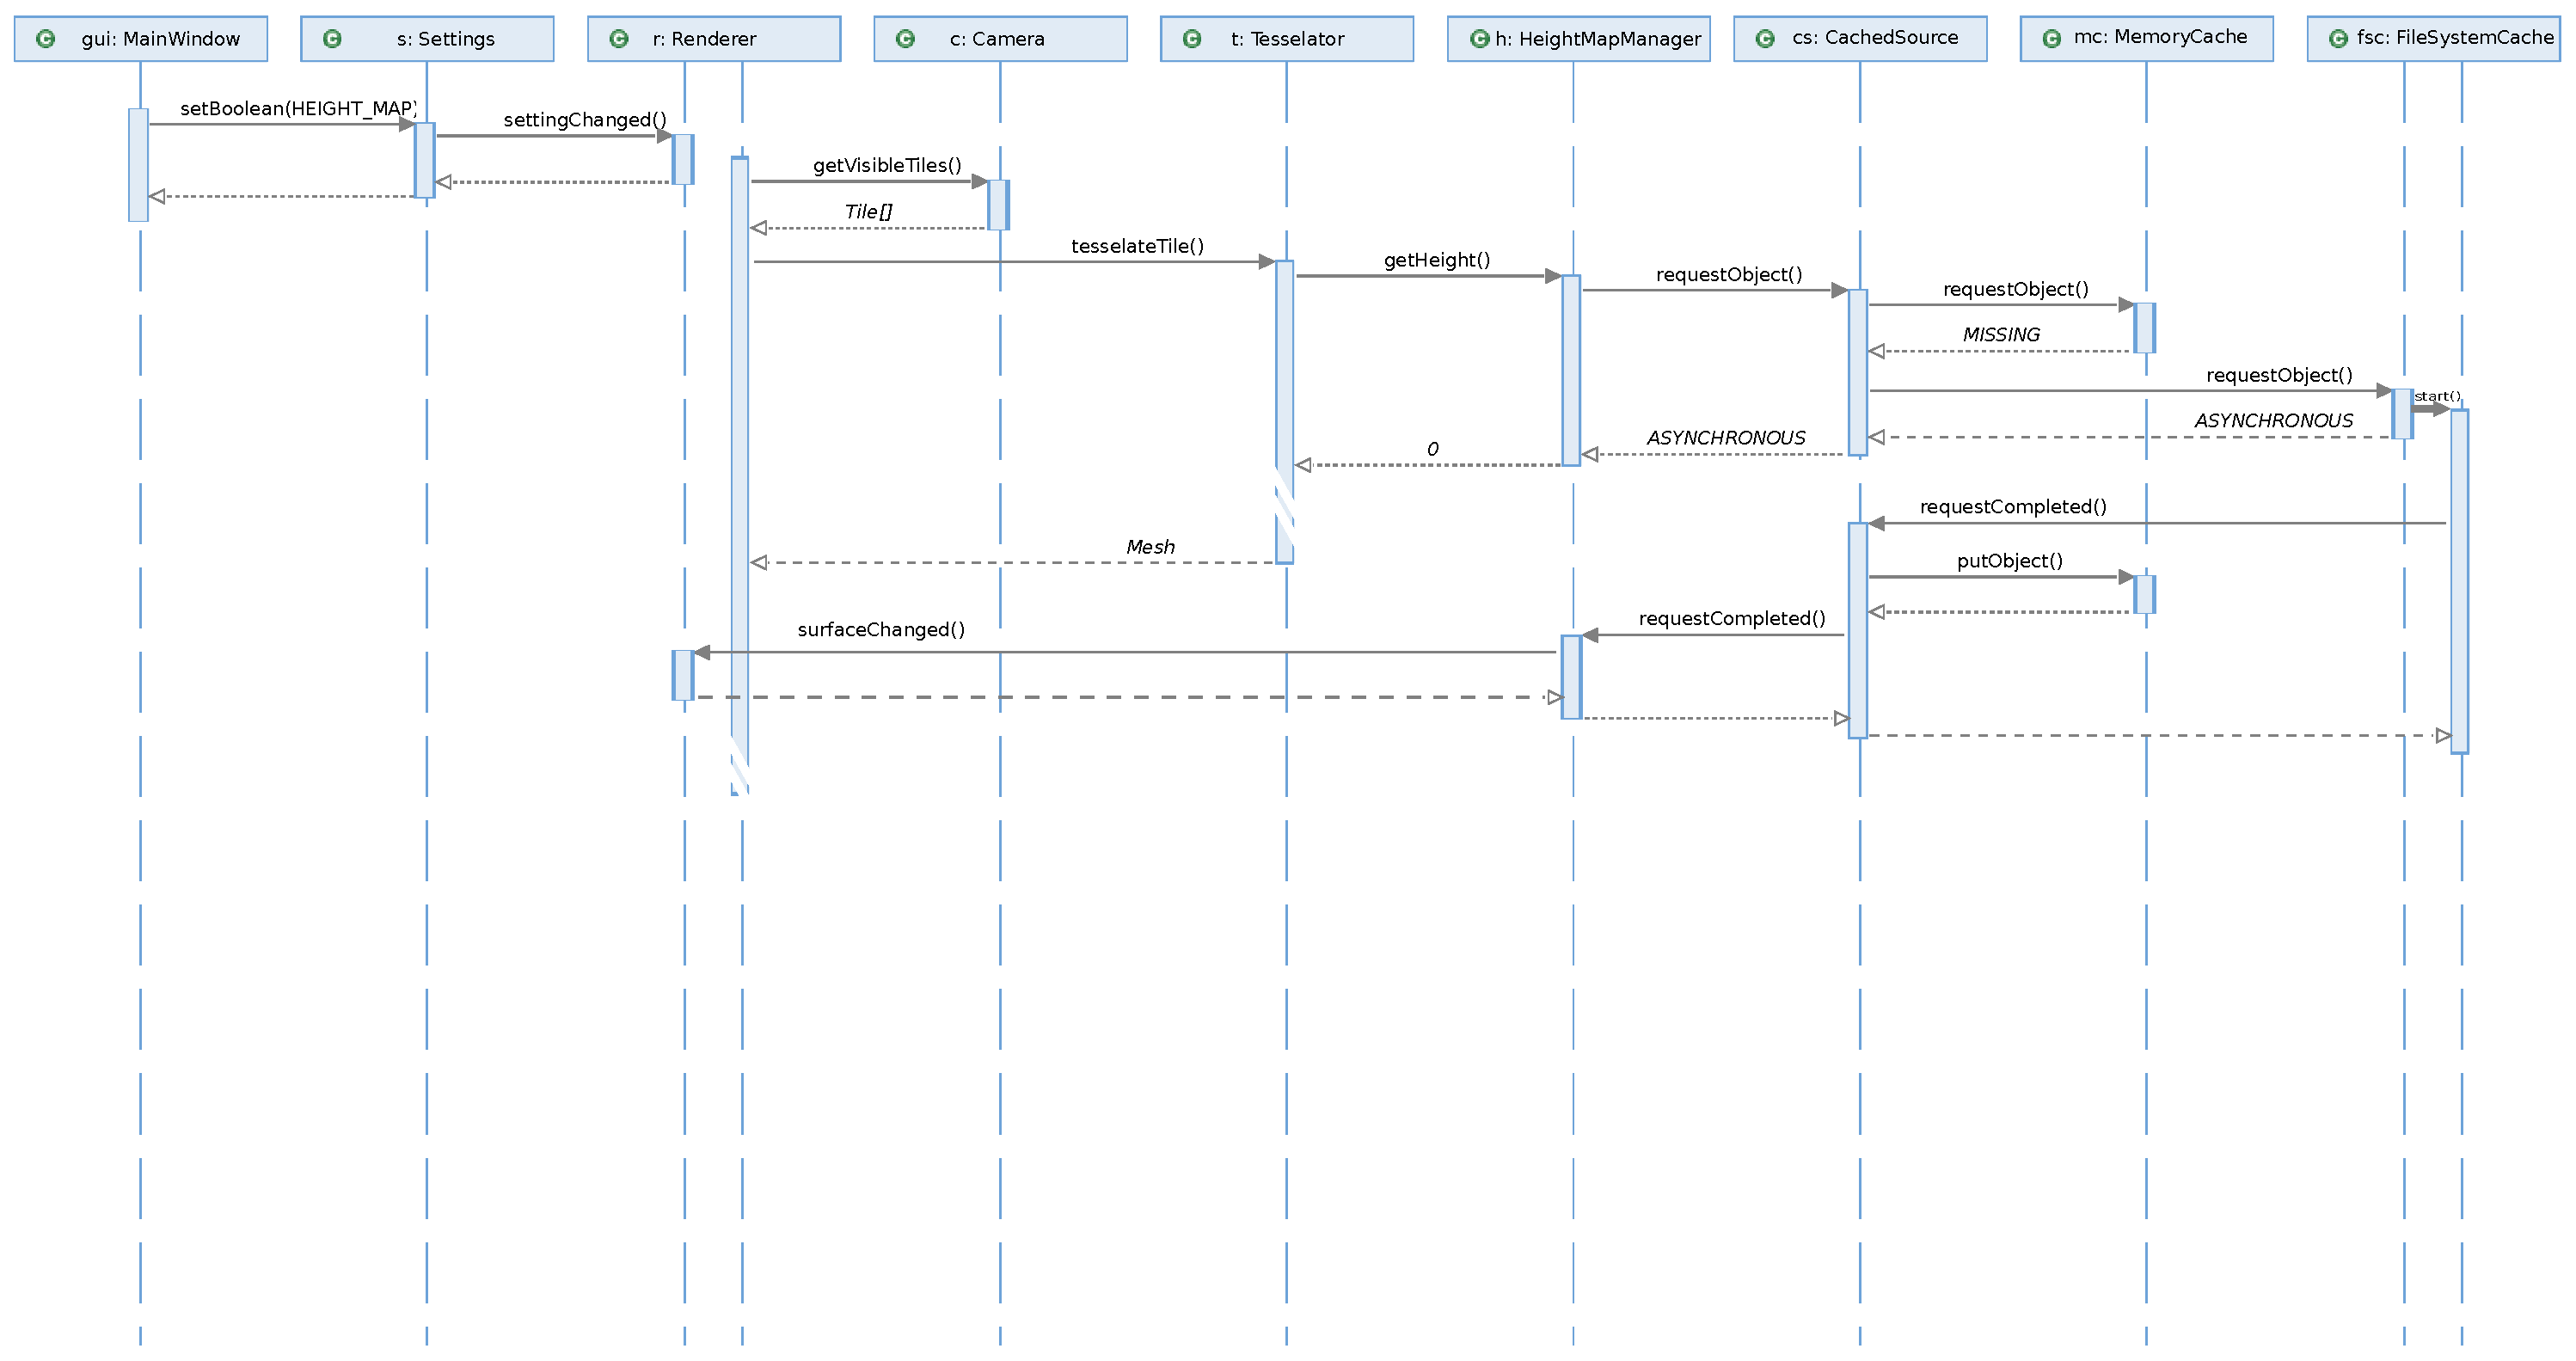
\includegraphics[scale=0.28]{sequenz-height.eps}
\caption{Aktivieren des Höhenprofils; Nachladen benötigter SRTM-Daten}
\end{center}
\end{figure}

\begin{itemize}
\item Im \textit{MainWindow} wurde die HeightMap Einstellung aktiviert, was dem \textit{Renderer} über die \textit{Settings} mitgeteilt wird, welche er beobachtet.
\item Dieser fordert in einem neuen Thread bei der \textit{Camera} die sichtbaren Kacheln an und übergibt diese dem \textit{Tesselator}.
\item Der \textit{Tesselator} fordert bei dem \textit{HeightMapManager} die Höhen an, die -analog zum obigem Diagramm- geladen werden.
\item Der \textit{Renderer} wird danach aufgefordert ein neues Bild zu zeichnen, da die Höhen nun vorliegen.
\item Dieser fordert wieder die sichtbaren Kacheln von der \textit{Camera} an, die anschließend an den \textit{Tesselator} zur Verarbeitung übergeben werden.
\item Der \textit{Tesselator} fordert die HeightMaps vom \textit{HeightMapManager} an und generiert aus diesen Informationen ein \textit{Mesh}, das er an den \textit{Renderer} zurückgibt.
\end{itemize}

\section*{Semantik der Diagramme}
\begin{itemize}
\item Senkrechte gestrichelte Linien enthalten sequentielle Aufrufe (\textit{Lebenslinien}). Gibt es zu einem Objekt oder einer Klasse mehrere solcher Linien, bedeutet dies, dass Aufrufe parallel in verschiedenen Threads ausgeführt werden.
\item Threads werden mit der asynchronen Nachricht \texttt{start()} angestoßen. Sie können beispielsweise mit einem \textit{ExecutorService} implementiert werden, der einzelne asynchrone Aktionen ausführen kann.
\item Blau-weiß diagonal unterbrochene Lebenslinien zeigen an, dass an dieser Stelle weiter Aufrufe vor Rückkehr der Funktion stattfinden, die aber für den Ausschnitt des Sequenzdiagramms keine Rolle spielen.
\end{itemize}


\chapter{Design Patterns}

\section{Systemarchitektur: Model-View-Controller}

Das \textit{Model-View-Controller Pattern} ist ein Architekturmuster.\\ Die zugrundeliegende Architektur des Programms wurde anhand des MVC-Patterns strukturiert.\\
\begin{figure}[ht]
\begin{centering}
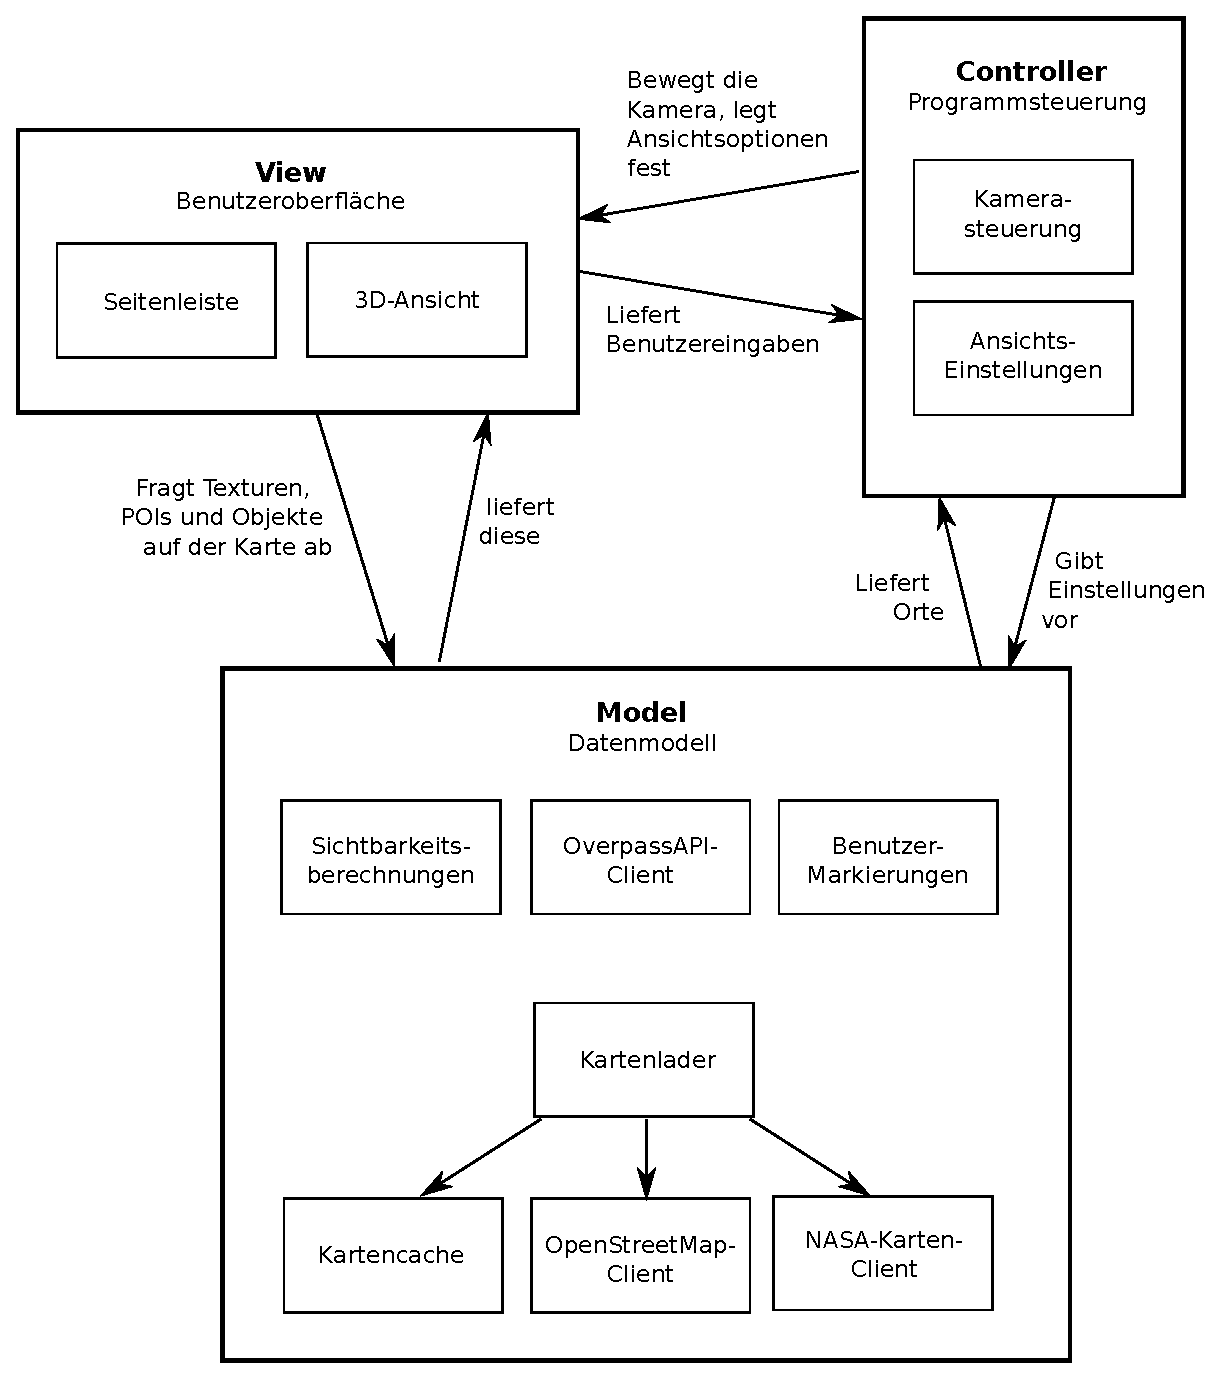
\includegraphics[scale=0.5]{ModelViewController.eps}
\caption{Das Model-View-Controller Pattern}
\end{centering}
\end{figure}

\newpage

\section{Weitere verwendete Entwurfsmuster}

\subsection{Adapter Pattern}
Das \textit{Adapter Pattern} ist ein Strukturmuster. \\
Es dient zur Übersetzung einer Schnittstelle in eine andere. \\ Dieses Pattern findet Anwendung bei den \textit{Mouse- und Key"-listenern}, welche in der Benutzeroberfläche implementiert werden. \\ Ziel ist es den Quellcode übersichtlich zu halten. Aus diesem Grund werden nur die benötigten Methoden der Listener überschrieben. Alle nicht erforderlichen Methoden werden ignoriert.

\subsection{Chain of Responsibility Pattern}
Das \textit{Chain of Responsibility Pattern} (bzw. Zuständigkeitskette) ist ein Verhaltensmuster. \\
Hierbei werden mehrere Objekte hintereinander verkettet um gemeinsam eine eingehende Anfrage bearbeiten zu können. Dafür wird eine Anfrage entlang der Kette durchgereicht, bis ein Objekt die Anfrage beantworten kann. \\ Es findet Anwendung beim Speichermanagement. Eine Anfrage für eine benötigte Ressource wird immer an den \textit{RequestDistributor} gestellt. Die Anfrage wird entsprechend der Kette (\textref Sequenzdiagramm 6.2) durchgereicht bis sie bearbeitet werden kann. \\ Ziel ist die Entkopplung des Auslösers einer Anfrage mit seinem Empfänger.

\subsection{Data Transfer Object}
Das \textit{Data Transfer Object} ist ein Muster für eine objektrelationale Abbildung. \\
Hierbei werden mehrere Daten gebündelt als ein Objekt übertragen. \\ Es findet Anwendung bei Suchergebnissen und der Anfrage nach POIs. Alle Datensätze werden dann gebündelt übergeben und nicht jede Information seperat. \\ Ziel ist es die Daten zu strukturieren bzw. vollständig gruppierte Information zu einer Anfrage zu erhalten.

\subsection{Iterator Pattern}
Das \textit{Iterator Pattern} ist ein Verhaltensmuster.\\ Hierbei wird die verwendete Datenstruktur elementweise durchlaufen, ohne deren interne Anordnung preiszugeben.\\ Es findet Anwendung bei der Verdrängungsstrategie. Es werden die verschiedenen Caches elementweise durchlaufen um die entsprechenden Einträge zu verdrängen.\\
Ziel ist es die eingesetzten Datenstrukturen effizient zu durchsuchen.

\subsection{Mediator Pattern}
Das \textit{Mediator Pattern} ist ein Verhaltensmuster. \\ Hierbei fungiert der Vermittler als Kommunikationsschnittstelle zwischen Objekten in einem komplexen System.\\ Es findet mehrfache Anwendung im gesamten Programm, wie beispielsweise beim Speichermanagement, beim Rendering, usw. \\ Ziel ist lockere Kopplung. Es sollen nicht alle Objekt voneinander Kenntnis besitzen.



\subsection{Observer Pattern}
Das \textit{Observer Pattern} ist ein Verhaltensmuster. \\ Hierbei wird eine Info bei durchgeführten Änderungen am Objekt an alle abhängigen Komponenten weitergegeben. \\ Es findet beispielsweise Anwendung beim \textit{SettingsListener}, \textit{CameraListener}, \textit{SurfaceListener} usw. \\ 
Ziel ist lose Kopplung und zudem werden die abhängigen Objekte automatisch über Änderungen in Kenntnis gesetzt.

\subsection{Singleton Pattern}
Das \textit{Singleton Pattern} ist ein Erzeugungsmuster. \\ Hierbei wird sichergestellt, dass genau eine einzige Instanz eines Objekts existiert. \\ Es findet Anwendung bei den \textit{Settings}, von der nur eine Instanz existieren darf. \\ Ziel ist eine sichergestellte Zugriffskontrolle auf das Objekt.




\chapter{Qualitätsmerkmale}
\section{Entwurfsqualität}
Bei der Qualität des Entwurfs beziehen wir uns auf \textit{Robert Cecil Martins} Merkmalsdefinitionen \footnote{Robert Cecil Martin (2002). Agile Software Development: Principles, Patterns and Practices. Pearson Education.} die im Folgenden erläutert werden.

\subsection*{Anzahl an Klassen und Interfaces}
Die Anzahl aller Klassen inklusive abstrakter Klassen (sowie Interfaces) im gesamten Paket. Es dient als aussagekräftiger Indikator für die Erweiterbarkeit eines Pakets.

\subsection*{Afferente Kopplung}
Die Abhängigkeit anderer Pakete von einem Paket ist ein Maß für dessen Verantwortlichkeiten und dessen Einfluss.

\subsection*{Efferente Kopplung}
Die Abhängigkeit eines Pakets von anderen Paketen ist ein Maß für die Unselbstständigkeit dieses Pakets.

\subsection*{Abstraktheit}
Der Anteil abstrakter Klassen (sowie Interfaces) an allen Klassen im Paket ist ein Indikator für die Abstraktheit eines Pakets.

\subsection*{Stabilität}
Das Verhältnis von afferenter Kopplung zur gesamten Kopplung gibt Auskunft über die Resilienz gegenüber Änderungen eines Pakets.

\subsection*{Balance von Abstraktion und Abhängigkeit}
Der Abstraktionsgrad der Klassen sollte in etwa deren Unabhängigkeit von anderen Klassen entsprechen. Bei Erfüllung der Anforderung spricht man von optimaler Balance.

\subsection*{Kohäsion}
Als Ergänzung zu Martin's Definitionen, welche sich nur auf das Zusammenspiel zwischen den Paketen bezieht, wird zudem die Kohäsion berücksichtigt.\\

Kohäsion ist der Versuch, zusammenhängende Programmstrukturen in einer Klasse zusammenzuführen, um z.B. nachträgliche Änderungen auf lokale Anpassungen des Codes zu beschränken.


\section{Gütekriterien nach ISO/IEC 9126}
\subsection*{Funktionalität}
Funktionalität beinhaltet Angemessenheit, Richtigkeit, Interoperabilität, Ordnungsmäßigkeit und Sicherheit.

\subsection*{Zuverlässigkeit}
Eine Menge von Merkmalen, die sich auf die Fähigkeit einer Software/eines Systems beziehen, ihr/sein Leistungsniveau unter festgelegten Bedingungen über einen festgelegten Zeitraum oder über eine festgelegte Anzahl von Transaktionen zu bewahren. [ISO 9126]

\subsection*{Benutzbarkeit}
Die Fähigkeit eines Softwareprodukts, unter spezifizierten Bedingungen für einen Benutzer verständlich, erlernbar, anwendbar und attraktiv zu sein. [ISO 9126]

\subsection*{Effizienz}
(1) Die Fähigkeit eines Softwareprodukts, unter festgelegten Bedingungen eine angemessene Leistung zu erbringen, bezogen auf den Umfang der eingesetzten Betriebsmittel. [ISO 9126]

\subsection*{Änderbarkeit}
Mit Änderbarkeit bezeichnet man den Aufwand, der zur Durchführung bestimmter Änderungen notwendig ist. Änderungen können Korrekturen, Verbesserungen oder Anpassungen an Änderungen der Umgebung, der Anforderungen und der funktionalen Spezifikation einschließen. [ISO 9126]

\subsection*{Portabilität}
Portabilität oder Übertragbarkeit ist die Eignung einer Software, von einer Umgebung in eine andere übertragen zu werden. Diese Umgebung kann die organisatorische Umgebung, Hardware- oder Software-Umgebung einschließen. [ISO 9126]

\newpage
\pagestyle{empty}

\newgeometry{top=30mm, left=25mm, right=25mm, bottom=20mm}

\chapter{Anhang}
\centering
\thispagestyle{empty}
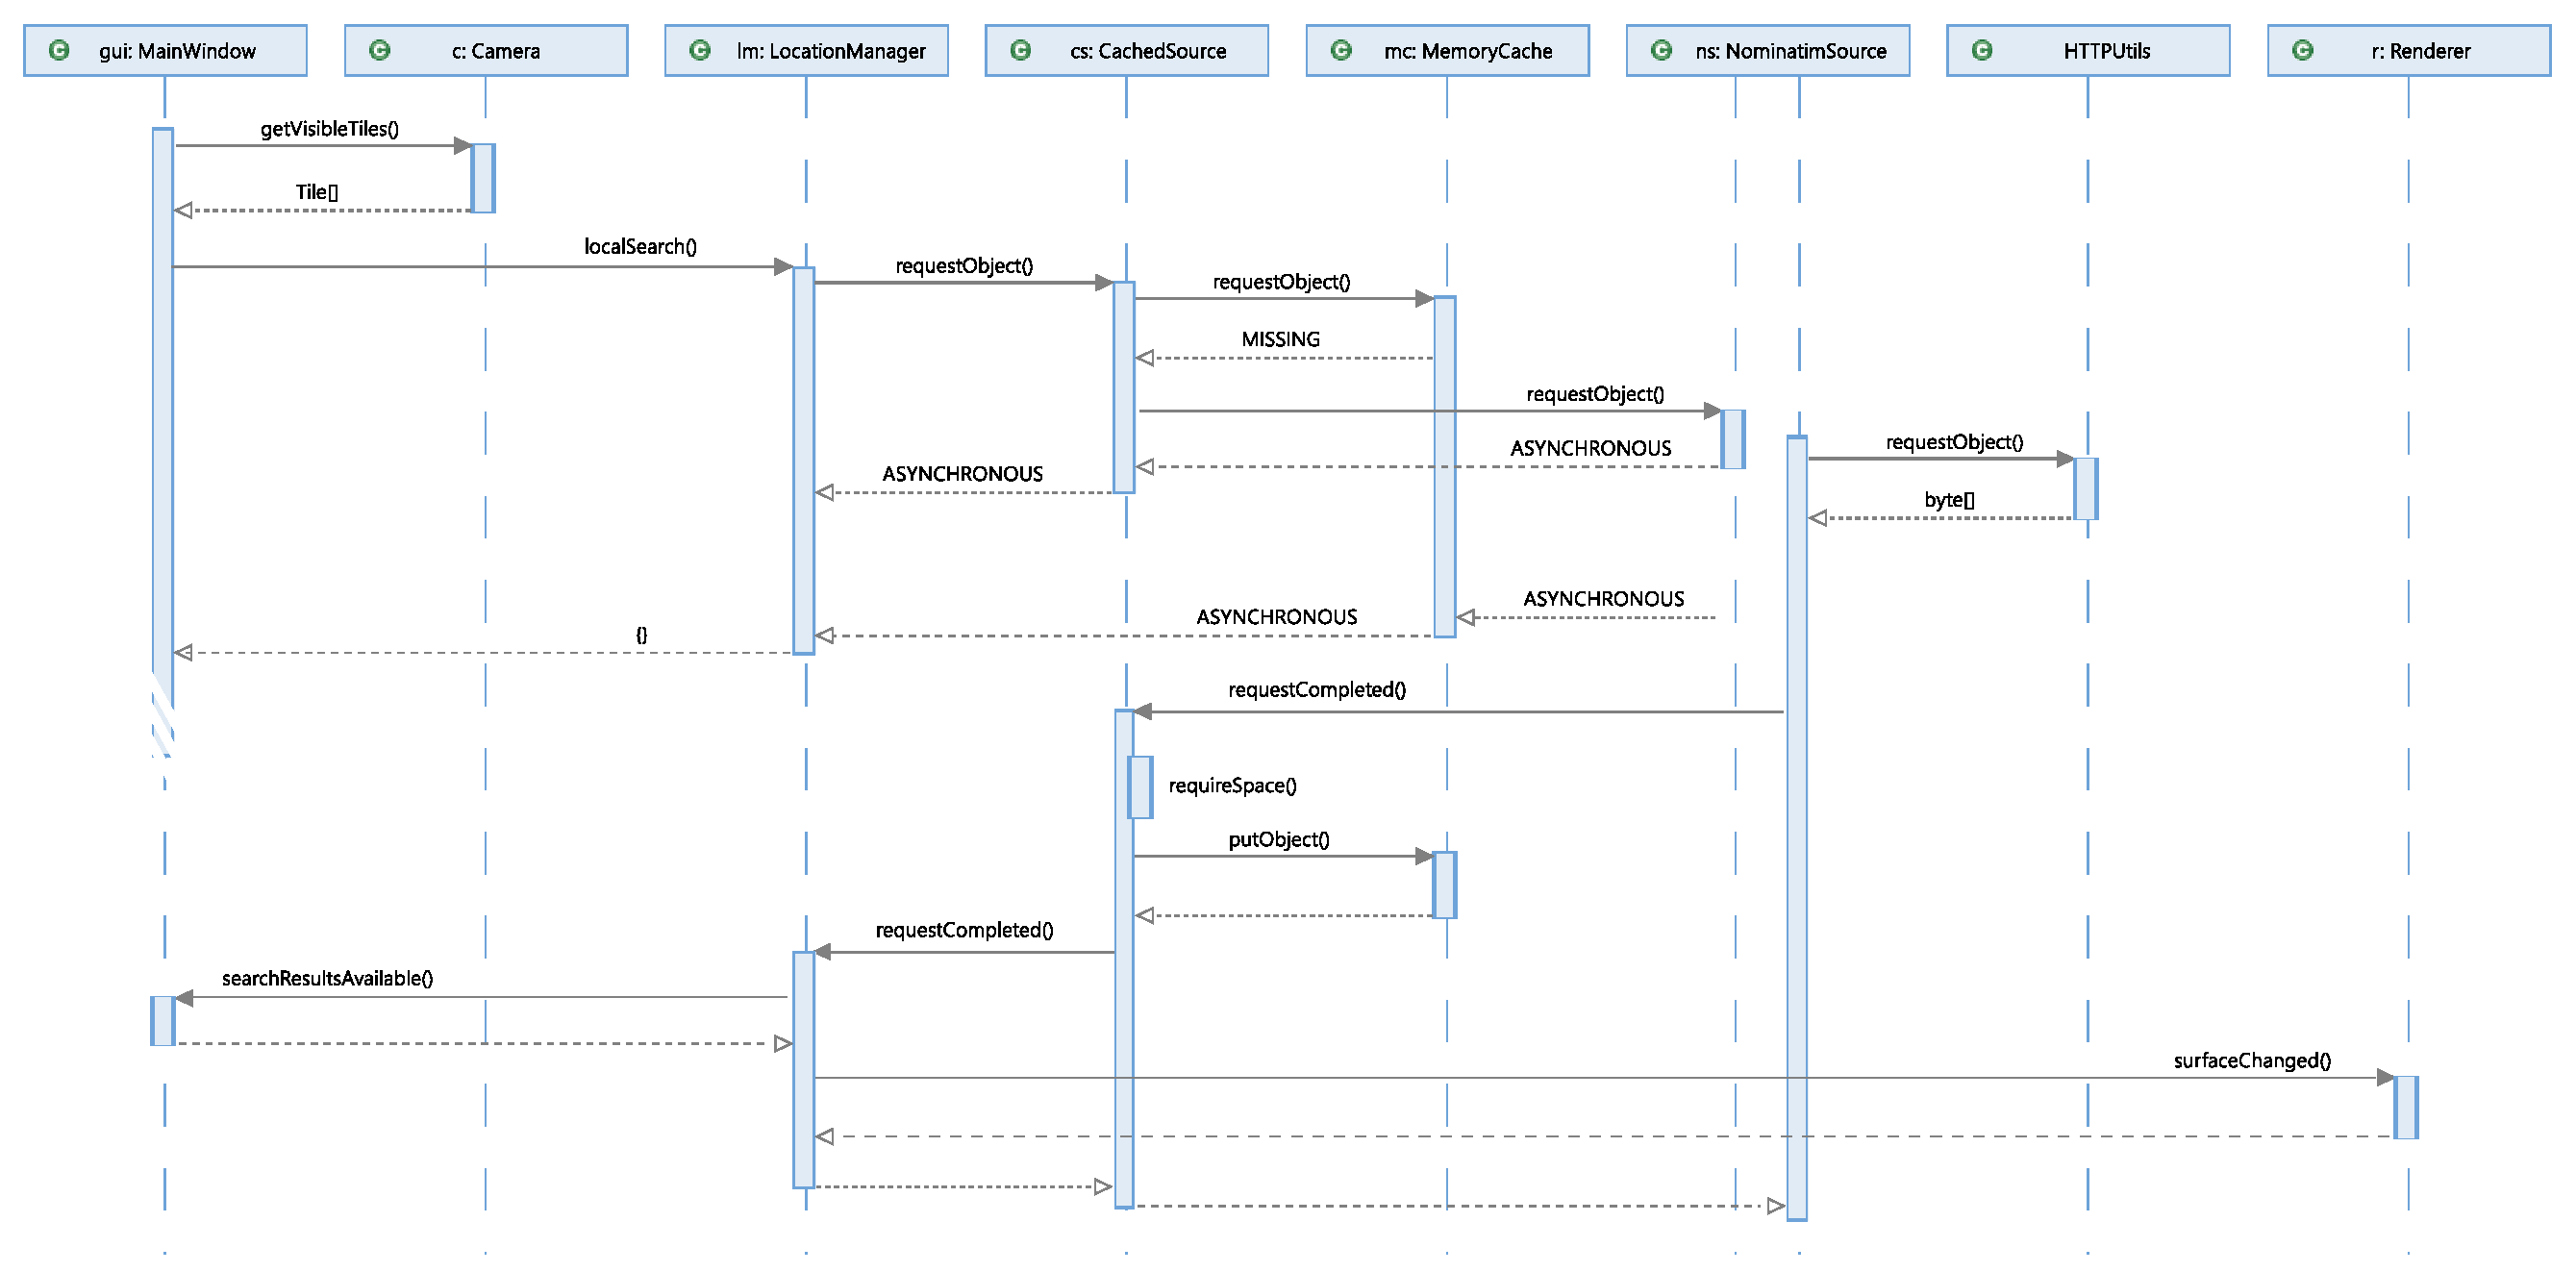
\includegraphics[scale=0.45,angle=90,origin=c]{sequenz-search.eps}
\hspace{5mm}
\begin{rotate}{90}
\textbf{Abbildung 9.1:} Lokale Suche nach einem Begriff
\end{rotate}

\newpage
\newgeometry{top=20mm, left=25mm, right=25mm, bottom=20mm}
\thispagestyle{empty}
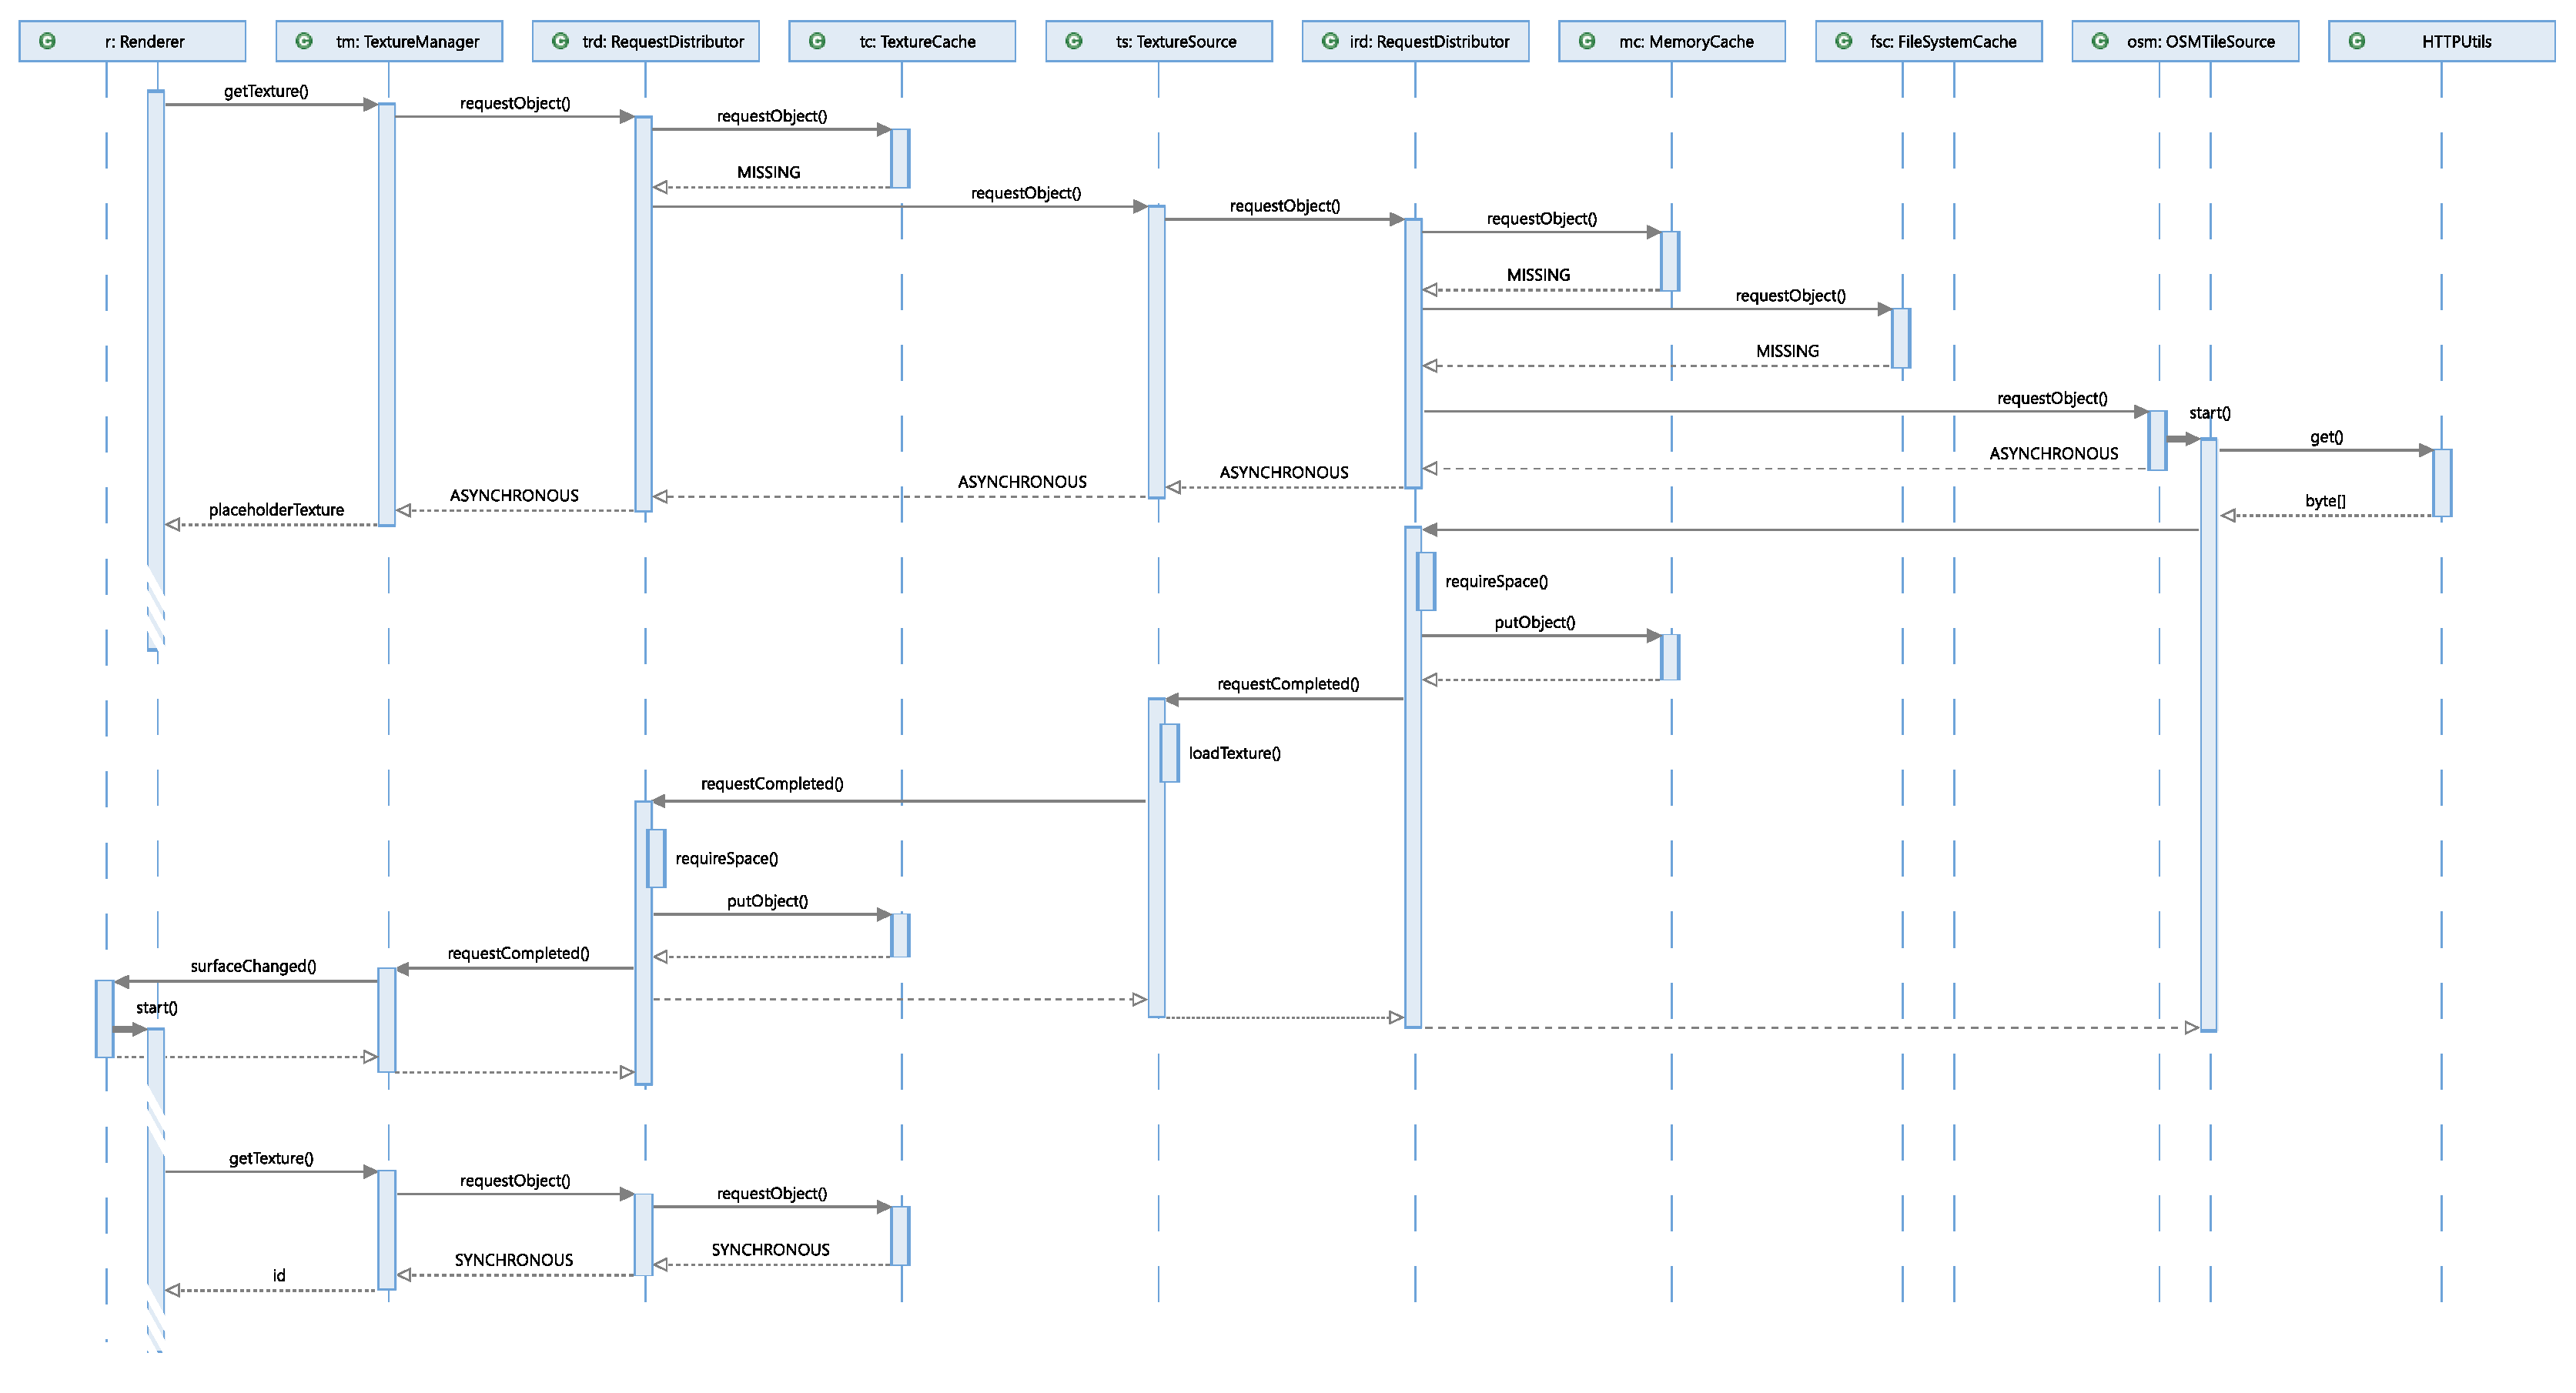
\includegraphics[scale=0.45,angle=90,origin=c]{sequenz-osmtile.eps}
\hspace{5mm}
\begin{rotate}{90}
\textbf{Abbildung 9.2:} Laden einer lokal noch nicht vorhandenen Kachel
\end{rotate}

\newpage
\thispagestyle{empty}
\vspace*{1cm}
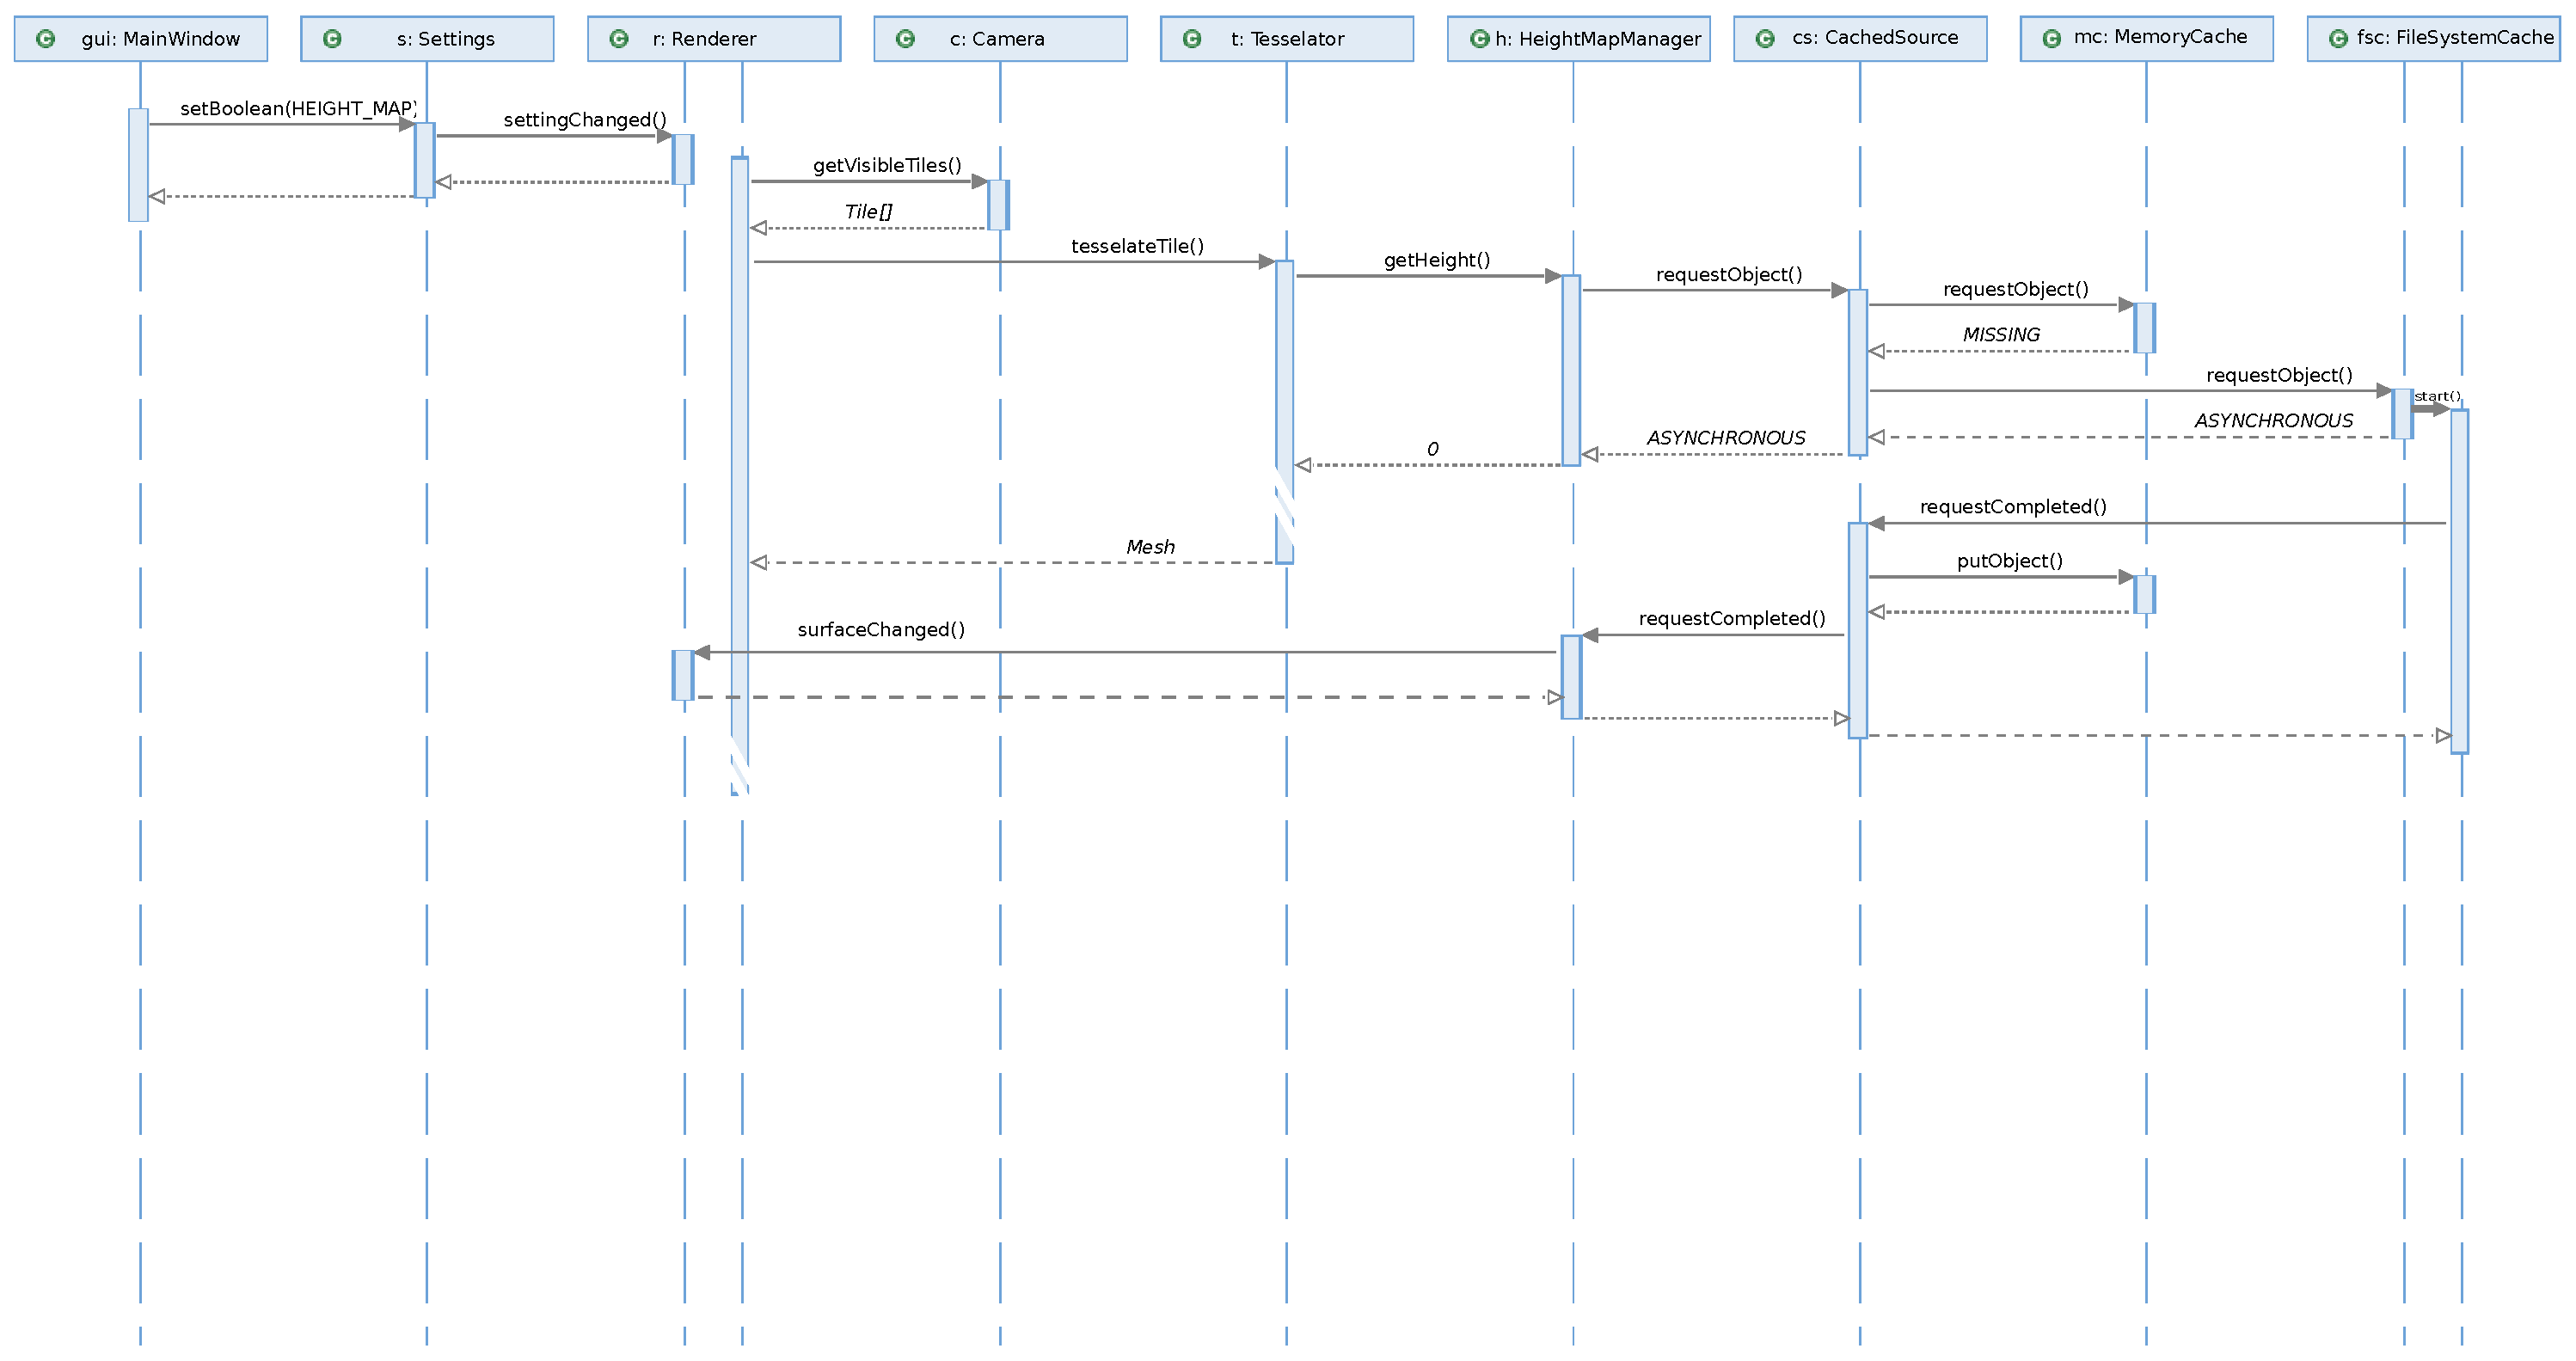
\includegraphics[scale=0.45,angle=90,origin=c]{sequenz-height.eps}
\hspace{5mm}
\begin{rotate}{90}
\textbf{Abbildung 9.3:} Aktivieren des Höhenprofils; Laden benötigter SRTM-Daten
\end{rotate}

\restoregeometry

\end {document}